\documentclass[]{kththesis}
\usepackage{csquotes} % Recommended by biblatex
\usepackage[style=numeric,sorting=none,backend=biber]{biblatex}
\usepackage[swedish]{babel}
\usepackage[]{graphicx}
\usepackage{float}


\graphicspath{{../images/}}

\addbibresource{references.bib}
\title{Image Classification of real estate images with transfer learning}
\alttitle{Bildklassificering av fastighetsbilder med transfer learning}
\author{Oskar Råhlén och Sacharias Sjöqvist}
\email{orahlen@kth.se och sacsjo@kth.se}
\supervisor{Handledare}
\examiner{Examinator}
\programme{Degree project in Computer Science}
\school{School of Electrical Engineering and Computer Science}
\date{\today}

% Uncomment the next line to include cover generated at https://intra.kth.se/kth-cover?l=en
% \kthcover{kth-cover.pdf}
% källor: \textcite och \parencite

\begin{document}
\frontmatter
\titlepage

\begin{abstract}
    English abstract goes here
\end{abstract}

\begin{otherlanguage}{swedish}
  \begin{abstract}
    Svenskt sammanfattning
  \end{abstract}
\end{otherlanguage}
  
\tableofcontents

\mainmatter

\chapter{Introduktion}
Koppla första mening till titel. söka på speicfika saker i en annons. mysig inledning. Deeplearning bildanalys - google grejer. Ai och hur automatisering vuxit fram. Lite fakta på hur viktig sökfunktioner är för att hitta bostäder? Hur många sökningar /tidsenehet. Om folk enklare hittar bostad på ett mer effektivt sätt så effektiviseras hela köp och sälj processen och därmed hela marknaden.

Just nu (april 2019) finns över 20 000 bostadsrätter (https://www.hemnet.se/statistik) till salu på Sveriges största mäklarsite (https://www.hemnet.se/om), där nästan hälften av dessa ligger i Stockholm. 
Dit kommer 2,8 miljoner (https://www.hemnet.se/om) unika besökare varje vecka och gör tillsammans över 2000 sökningar i minuten.
Detta ställer höga krav på filtreringsfunktionerna för att potentiella köpare snabbt ska kunna hitta sin drömbostad.
Idag erbjuds redan filtreringsfunktionerna ”antal rum”, ”boarea”, ”pris” samt ”område”. 
Det finns också en fritextsöka där man kan söka på vad mäklaren har skrivit i texten.
Exempel på sökord är ”balkong”, ”kakelugn” och ”sjöutsikt”. 

Problemet med att söka i mäklartexter är att det tvingar mäklaren att i texten nämna samtliga attribut som han eller hon vill göra sökbara. 
Detta gör att vissa attribut kan bli utelämnade vilket i sin tur gör fritextrutan sämre.

Exempelvis är det ofta självklart om det finns en balkong eller kakelugn på mäklarbilderna men det är inte alltid mäklaren väljer att skriva detta i den löpande texten.
Det hade därför varit intressant att utifrån mäklarbilderna automatiskt generera ett sökindex där varje bild knyts till ett antal attribut.
Dessa attribut skulle sedan kunna användas för att lägga till filtreringsalternativ i sökfunktionen och därmed skapa en bättre användarupplevelse.

Det skulle också gå att använda sig av denna metod för att knyta attribut såsom skick och typ av rum (Sovrum, badrum eller kök) till varje bild.
Kombinationen skulle göra sökningar såsom ”Kök i gott skick” möjligt.  

Denna data kan också vara användbar vid värdering av bostäder, då det enkelt skulle gå att jämföra priser på bostäder med olika attribut, tillexempel lägenheter med sköutsikt mot lägenheter utan sköutsikt eller lägenheter med ett kök i gott skick mot lägenheter med ett kök i sämre skick.

VET INTE RIKTIGT HUR JAG SKA FORMULERA MIG HÄR!! Känns Som ett halvbra stycke
För att på ett effektivt och precist sätt kunna knyta attribut till mäklarbilder behöver man använda sig av någon form av automatisk bildbehandling.
Detta går att göra med hjälp av maskininlärning och djupa neurala nätverk.
Sättet som detta görs på är att man tränar ett antal bilder som innehåller det givna attributet och ett antal som inte innehåller attributet.
Modellen tränas sedan med hjälpt av ett djupt neuralt nätverk. 
Efter varje träning så testas modellen för att mäta hur många träningar som krävs för bästa resultat.
När modellen är färdigtränad kan man använda denna genom att skicka in en bild som input och modellen berättar om bilden innhåller attributet eller inte.

\section{Syfte}
Syftet med denna studie är att titta på hur olika maskininlärningsmetoder kan användas för att hitta relevanta nyckelord till bilder på lägenhetsannonser. 

\section{Frågeställning}
Går det med nuvarande verktyg inom maskininlärning hitta attribut i bilder från lägenhetsannonser?

\section{Avgränsningar}
För att sätta en rimlig avgränsningar på denna uppsats kommer tre olika sorters attribut undersökas och jämföras med tre olika sorters deeplearningmodeller. 
Attributen som kommer– användas är ”Balkong”, ”Kakelugn” samt ”Typ av rum” (Kök, badrum eller sovrum) och deelearningmodellerna som kommer användas är ”keras”, ”smartAI”, samt ”blabla”. 
Anledningen till att flera attribut eller flera sorters modeller inte valdes är att det är resurskrävande att både samla in och sortera testdata samt att implementera modellerna. 
Anledningen till att färre inte valdes var för att få spridning på attributen och modellerna, för kunna svara på om klassifiseringen fungerar i allmänhet och inte bara i enstaka testfall. 
En annan avgräsning som gjort är att mäklarbilderna som används endast kommer från bostadsrätter, då det kan skilja sig ganska mycket på hur villor och bostadsrätter ser ut.

\chapter{Bakgrund}

\section{Maskininlärning}
Maskininlärning är ett sätt att programmera datorer så de optimerar ett problem med hjälp av exempeldata eller tidigare erfarenhet \parencite{alpaydin2009introduction}. Maskininlärning är ett aktivt forskningsfält inom datalogi. Lärandeprocessen för en maskininlärningsalgoritm kan se ut på följande sätt: Ett datorprogram har som uppgift att lära sig en förutbestämd uppgift T, hur väl den gör detta, algoritmens prestanda, är måttet P. Till sin hjälp har datorprogrammet tidigare erfarenhet E. Om prestandan P blir högre då vi tillhör erfarenheten E till programmet, då lär sig programmet.

Maskininlärningsmodeller kan delas in i två kategorier, övervakat lärande (eng. supervised learning) och oövervakat lärande (eng. unsupervised learning) \parencite{murphy2012machine}. Vid övervakat lärande så är erfarenheten E redan kategoriserad och uppmärkt för uppgiften T, vid oövervakat lärande så är den inte det. Ett exempel är en maskininlärningsmodell som har som uppgift T att kategorisera bilder i vissa förutbestämda kategorier. Vid övervakat lärande kommer erfarenhet E bestå av bilder som redan är uppmärkta med rätt kategori. Modellen ska då med hjälp av erfarenheten kunna kategorisera ny data som inte är uppmärkt. 

\section{Artificella neurala nätverk}
En samling algoritmer inom maskininlärning med många tillämpningsområden är artificella neurala nätverk (ANN). Enligt \textcite{Goodfellow-et-al-2016} så var från början ANN ett försök till att bygga en digital modell av det biologiska neuronsystemet. Forskningen inom områden avvek dock snabbt från att efterlikna den biologiska varianten och fokuserade istället på att öka prestandan på maskininlärningsproblem. De minsta byggstenarna i ANN, neuronen, fungerar fortfarande som dess biologiska variant. En neuron får signaler in och skickar sedan signaler ut via synapserna. Hur stark utsignal bör vara simuleras i en dator med hjälp av vikter (eng. weights), även kallat för parametrar. Varje neuron i nätverket har sina tillhörande vikter. När ett ANN tränas så görs detta genom att justera dessa vikter \parencite{Goodfellow-et-al-2016}. De viktade insignalerna bör även nå upp till en viss tröskel för att en utsignal ska skickas, detta simuleras i ANN med aktiveringsfunktioner. ANN är en acyklisk graf som består av dessa artificiella neuroner.

\begin{figure}[h]
  \centering
  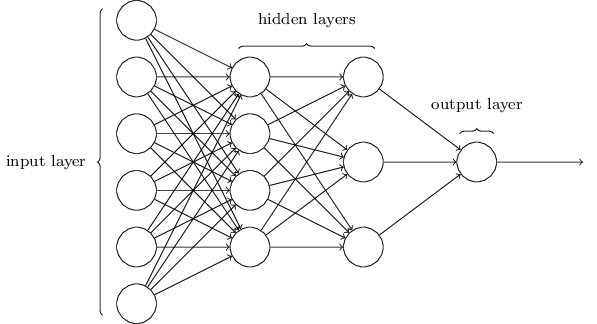
\includegraphics[width=0.6\textwidth]{nn}
  \caption{En illustration över ett artificiellt neuralt nätverk \parencite{nielsen2015neural}.}
\end{figure}

Ett ANN består först av ett indatalager (eng. input layer). Indatalagret representeras av en neuron per kännetecken (eng. features) i indatan. Då indata är bilder motsvarar en neuron i indatalagret en pixel i bilden. Indatalagret är sedan ihopkopplat med ett nytt lager med neuroner. Det kan vara flera lager efter varandra och dessa kallas för de gömda lagren (eng. hidden layers). De gömda lagren kan bestå av godtyckligt många neuroner och de behöver inte ha samma antal neuroner. Efter de gömda lagren kommer utdatalagret (eng. output layer). Antalet neuroner i utdatalagret bör motsvara formen på den utdata vi vill ha. Om modellen ska kategorisera bilder i tio olika kategorier, bör utdatalagret innehåller tio neuroner. Det är värdet dessa neuroner i utdatalagret har som är svaret från vårt ANN.

Ett ANN blir bättre på att utföra sin uppgift genom att ändra sina vikter. Detta sker i två steg, feed-forward pass och backward pass, även kallat för backpropagation \parencite{alpaydin2009introduction}. Vid feed-forward skickas träningsdata (som kommer från tidigare erfarenhet E) in i nätverket för att få ut ett svar. Då träningsdatan är uppmärkt så jämförs svaret från nätverket med det korrekta svaret. Utifrån antal fel och hur fel nätverket hade, beräknas en kostnad. Denna kostnad kan beräknas på olika sätt men vanligtvis används funktionen cross-entropy loss \parencite{Goodfellow-et-al-2016}. Målet är att träna modellen så denna kostnad blir så låg som möjligt. Nästa steg är backward pass. Vi vill ändra vikterna så att kostnaden blir lägre, detta görs genom att beräkna gradienten av kostnaden med avseende på alla vikter. Vi tar sedan ett steg åt motsatt håll till gradienten för att minska kostnaden. Storleken på detta steg kallas för inlärningstakt (eng. learning rate).

Vanligtvis delas träningsdatan in i högar, vilket kallas för mini-batch \parencite{Goodfellow-et-al-2016}. Istället för att beräkna gradienten för varje datapunkt i träningsdatan så beräknas gradienten för en hel mini-batch för att sedan använda sig av en genomsnittlig gradient. En epok (eng. epoch) är när nätverket har gått igenom alla datapunkter i träningsdatan. Hur många träningssteg detta innefattar beror på antal datapunkter samt storleken på mini-batch.

\subsubsection{Stochastic gradient descent}
Det finns olika algoritmer för exakt hur vikterna ska ändras när ett ANN tränas. En av de vanligaste algoritmerna är Stochastic Gradient Descent (SGD) \parencite{Goodfellow-et-al-2016}. Den bygger på feed-forward pass och backward pass men beräknar gradienten på ett fåtal slumpmässigt utvalda datapunkter istället för alla datapunkter i träningsdatan \parencite{bottou2010large}. Anledningen är att effektisera modellen så träningen går snabbare. En variant är mini-batch SGD, där samma principer appliceras på en mini-batch istället för på hela träningsdatan.

En vidareutveckling är SGD med momentum \parencite{qian1999momentum}. Algoritmen med momentum kommer ihåg förändringen av vikterna vid föregående iteration och baserar nästa uppdatering på en linjärkombination av gradienten och den tidigare förändringen. Denna teknik har fått stor genomslagskraft inom forskningen av ANN \parencite{sutskever2013importance}.

\section{Neurala nätverk med konvolution}
Neurala nätverk med konvolution (eng. Convolutional Neural Network, CNN) är en viss typ av neurala nätverk som fungerar bra då indatan kan ses som ett rutnät \parencite{Goodfellow-et-al-2016}. Detta inkluderar data om tidsserier, som kan ses som ett endimensionellt rutnät, men också bilder, som kan ses som ett rutnät av pixlar. CNN introducerades för 20 år sedan men det har, på grund av begränsningar i hårdvara och arkitekturer, inte gått att träna djupa CNN förrän för några år sedan \parencite{huang2017densely}. Enligt \textcite{huang2017densely} har CNN idag blivit den dominanta tekniken inom maskininlärning för igenkänning av visuella objekt. Och enligt \textcite{simon2016imagenet} är CNN som är förtränade på bilder från ImageNet grunden till majoriteten av state-of-the-art-modeller inom bildkategorisering.

\subsection{Lager}
Det finns några grundläggande lager som används i de flesta typer av CNN, oberoende av arkitektur. CNN kan användas för många olika typer av indata men vi har här valt att fokusera på dess tillämpningar med bilder. En vanlig uppbyggnad av ett CNN för bildkategorisering är indatalager, konvolutionslager, ReLU, föreningslager och sist ett FC-lager.

\subsubsection{Indatalager}
Detta lager innehåller pixelvärden från bilden som skickas in i nätverket. Vanligtvis används RGB-bilder, vilket betyder att varje pixel även har tre färgkanaler. Storleken på bilden beror på arkitektur men vanligast är formatet som används i ResNet-arkitekturen, vilket är 224 pixlar i höjd och 224 pixlar i bredd \parencite{krizhevsky2012imagenet}. Storleken på tensorn som innehåller indata motsvarande en bild har då storleken 224 x 224 x 3. Alla arkitekturer som fått större spridning tar alltid en kvadratisk bild som indata.

\subsubsection{Konvolutionslager}
En konvolutionslager består av en godtycklig mängd filter med träningsbara vikter \parencite{lecun1995convolutional}. Varje filter är kvadratiskt och brukara vara små i höjd och bredd med samma djup som indatan till lagret. Ett exempel på filterstorlek är 5 x 5 x 3 \parencite{krizhevsky2012imagenet}. Vid feed-forward pass så glider vi detta filter över bilden som är vårt indata. Vi beräknar skalärprodukten av filtret och den mängd pixlar av bilden som filtret ligger över. Efter beräkningen glider vi filtret åt sidan \parencite{he2015spatial}. Vanligtvis skjuts filtret en pixel i taget, men det kan skilja mellan lager. Utdata från varje filter blir en tvådimensionell aktiveringskarta (eng. activation map). Höjd och bredd på utdatan från ett konvolutionslager beror på tre hypterparametrar: Antal filter, kliv (eng. stride) och nollutfyllnad (eng. zero padding). Antal filter motsvarar djupet på utdatan. Kliv bestämmer antal pixlar vi förflyttar oss vid varje glidning och nollutfyllnad avgör om vi skapar en ram runt indatan med nollor och i sådana fall hur tjock den ramen är. Klivstorlek och nollutfyllnad avgör dimensionerna på utdata.

\subsubsection{Aktiveringslagret ReLU}
Aktiveringslagret (eng. activation layer) består av en aktiveringsfunktion. Denna funktion ska motsvara den tröskel som finns i biologiska neuroner för att trigga en utsignal. En av de vanligaste aktiveringsfunktionerna inom djupinlärning för bildkategorisering är Rectified Linear Units (ReLU) \parencite{krizhevsky2012imagenet}. Aktiveringsfunktionen appliceras elementvis och ReLU applicerar funktionen \begin{equation} f(x) = max(0,x) \end{equation} på varje element i indatan till lagret. Det betyder att varje element som är positivt är opåverkat och varje negativt värde får värdet noll. Storleken på datan blir oförändrad.

\subsubsection{Föreningslager}
Ett föreningslager (eng. pooling layer) applicerar en nedsampling (eng. downsampling) på indata \parencite{krizhevsky2012imagenet}. Detta sker längs de spatiala dimensionerna bredd och höjd. Vanligtvis sker detta för att minska antalet parametrar i nätverket och för att minska beräkningskrafen som behövs för att träna nätverket. Det är även en teknik för att undvika överanpassning (eng. overfitting). Det som främst används inom CNN är max pooling. Det är när ett förutbestämt område, till exempel 2 x 2 pixlar, sammanfattas genom att det högsta värdet av dessa fyra pixlar väljs ut. Max pooling med filter i storlek 2 x 2 och klivstorlek 2 är vanligt förekommande. Indata minskar då i storlek med 75\%.

\subsubsection{FC-lager}
Det lager som är vanligt förekommande i tradionella neurala nätverk är FC-lagret (eng. Fully-connected layer) \parencite{krizhevsky2012imagenet}. I detta lager har varje neuron en koppling till alla aktiveringar från det tidigare lagret. Dessa neuroner har tillhörande träningsbara vikter, som vanligtvis sparas i en matris \parencite{Goodfellow-et-al-2016}. Detta möjliggör även effektiva implementationer med matrismultiplikation. Storleken på utdata beror på storleken på viktmatrisen. I CNN är det vanligt förekommande att det sista lagret är ett FC-lager som byggs på det sättet att formen på utdata motsvarar antal kategorier modellen ska kunna kategorisera i. Ett exempel är att om en bild ska klassificeras bland tio klasser, så kan utdata från sista lagret ha formen 10 x 1.

FC-lager som används i slutet av nätverk brukar även kombineras med ett softmax-lager. Ett softmax-lager gör att de olika utdatavärdena kan ses som en distribution \parencite{Goodfellow-et-al-2016}.

\subsection{Tekniker inom djupinlärning}
Det har uppkommit vissa tekniker inom djupinlärning som inte är en del av artikekturer inom CNN men som ofta används med moderna modeller för att uppnå höga resultat. Två populära tekniker är batch-normalisering och dataförstärkning.

\subsubsection{Batch-normalisering}
Att träna djupa neurala nätverk är komplicerat då distributionen av varje lagers indatavärden förändras under träning \parencite{ioffe2015batch}. Detta leder till att träningen av nätverket tar längre tid, då vi behöver använda långsammare inlärningstakt. Det leder också till att viktinitieringen blir väldigt finkänslig. Enligt \textcite{ioffe2015batch} kallas detta fenomen för internal covariate shift och löses genom att normalisera indata till varje lager. Metoden bygger på att normaliseringen blir en del av arkitekturen och där en normalisering sker för varje mini-batch av vårt träningsdata. Denna typ av batch-normalisering tillåter oss att använda högre inlärningstakt och gör att initieringen av vikterna inte blir lika kritisk. Det fungerar även som regularisering (eng. regularization), vilket gör att andra tekniker för regularisering kan uteslutas.

Batch-normalisering har visat sig vara extra viktigt för lyckad träning och för att större nätverk ska konvergera, nätverk som VGG19 \parencite{simon2016imagenet}. Det har även visat sig att den högre inlärningstakten, som batch-normalisering tillåter, leder till en högre slutlig noggrannhet än vad som annars hade varit möjlig \parencite{simon2016imagenet}. Tidigare experiment har visat att detta har fungerat både bland annat AlexNey och VGG19 \parencite{simon2016imagenet}.

\subsubsection{Dataförstärkning}
Djupa neurala nätverk behöver en stor mängd data för att lära sig effektivt. Insamlingen av denna data är oftast dyrt och tidskrävande. Dataförstärkning (eng. data augmentation) löser detta genom att öka datamängden artificiellt genom att göra förändringar på befintlig data \parencite{taylor2017improving}. Det har visat sig att generell dataförstärkning leder till ökad prestanda på de flesta CNN. En viktig del av dataförstärkningen är att indata fortfarande ska tillhöra samma klass som den tillhörde innan. Inom bildkategorisering så sker förändringen med geometriska och fotometriska transformationer. Geometriska transformationer ändrar geometrin i bilden med målet att vårt CNN ska vara oberoende av objektets position eller orientering. Dessa transformationer inkluderar att flippa, beskära, skala och rotera bilden. Fotometriska transformationer förändrar istället färgkanalerna och målet är att vårt CNN ska vara oförändligt till skillnader i belysning och färg. 

\subsection{Arkitekturer}
Här presenteras ett urval av de mest betydelsefulla arkitekturerna inom CNN för bildkategorisering. En tydlig trend är att CNN har fått fler lager, blivit djupare, med tiden. Från LeNet \parencite{lecun1998gradient} med fem lager, till VGG med 19 lager \parencite{simonyan2014very} och Residual Networks (ResNet) med över 100 lager \parencite{he2016deep}. Ett problem med detta är att viktig information i indata försvinner innan det hinner nå slutet av nätverket \parencite{huang2017densely}. Det har därför kommit arkitekturer som försöker lösa detta problem. ResNet löser det genom att förbikoppla vissa lager med identitetskopplingar. DenseNet skapar istället flera olika förbikopplingar inne i nätverket.

\subsubsection{ResNet}
ResNet är en arkitektur för CNN som består av konvolutionslager, föreningslager och FC-lager \parencite{he2016deep}. ResNet finns i olika varianter, från ResNet18 till ResNet152, och skillnaden är storleken på nätverket, där ResNet18 består av 18 lager. Efter utvecklingen av djupare CNN så nådde till slut ett tak för hur kraftfulla modellerna kunde vara. ResNet är en lösning på det här problemet som introducerar identity shortcut connections. Det betyder att det finns kopplingar som hoppar över vissa konvolutionslager, vilket betyder att om nätverket tycker att vissa lager är onödiga så kan den helt enkelt skippa dessa. Anledningen till namnet är att dessa kopplingar skickar vidare indentiteten av indatan till nästkommande lager. Dessa kopplingar leder till att nätverken kan göras hur stora som helst utan prestandaförlust, för modellen kan alltid använda indentiteten. Modeller med dessa residuala funktioner ska även vara enklare att optimera \parencite{he2016deep}. ResNet-modellen tar RGB-bilder i storleken 224 x 244 pixlar som indata och målet är att kategorisera bilden bland 1000 kategorier från ImageNet. ResNet18 består först av ett konvolutionslager och sedan ett max pooling-lager. Därefter kommer en stack med konvolutionslager där det även sker en nedsampling med föreningslager. De sista lagren består av ett föreningslager av typen average pooling, ett FC-lager med utdata 1 x 1000 och ett softmax-lager.

\subsubsection{Alexnet}
Alexnet är en enklare variant av CNN, vann tävligen ILSVR 2012 och består av totalt åtta lager \parencite{krizhevsky2012imagenet}. De första fem lagrena är konvolutionslager, där vissa av dem även applicerar max pooling efteråt. De tre sista är FC-lager, där det sista har utdataformen 1 x 1000 för att motsvara klasserna i ImageNet. På detta sista FC-lager appliceras även softmax. Aktiveringsfunktionen i modellen är ReLU och indata består av RGB-bilder med storleken 224 x 244. Konvolutionslagren använder sig av filter i storlekarna 11 x 11, 5 x 5, 3 x 3. Nätverket tränades ursprunligen med SGD med momentum.

\subsubsection{VGGNet}
Enligt \cite{simonyan2014very} så har VGG högre noggrannhet än Alexnet och uppnådde år 2015 state-of-the-art noggrannhet på ILSVRCs klassificering och lokaliseringsuppgifter. Alla konvolutionslager i modellen följer samma design som de i Alexnet \parencite{simonyan2014very}. 

Enligt \cite{simonyan2014very} ser arkitekturen ut som följande: Under träning så består indata av RGB-bilder av fixerad storlek 224 x 224. Den enda förbehandlingen är att medelvärdet av RGB-värdena som beräknas på träningsmängden subtraheras från varje pixel. Bilden skickas sedan igenom en stack av konvolutionslager med filter av storlek 3 x 3. I en av konfigurationerna används även 1 x 1-filter, som kan ses som en linjär transformation av indatakanalerna. Klivstorleken är 1 pixel och nollutfyllnaden beror på filterstorlek, men ska se till att indata och utdata är i samma storlek. Exempelvis så är nollutfyllnaden 1 pixel vid 3 x 3-filter. Spatial pooling sker med fem stycken max-pooling lager efter vissa av konvolutionslager. Det är dock inte alla konvolutionslager som följs av max pooling. Max-pooling sker med ett 2 x 2-filter med klivstorlek 2. En stack av konvolutionslager, som är olika djup beroende på vilken typ av VGG, följs sedan av tre stycken FC-lager. De första två har 4096 kanaler var och det sista har 1000-kanaler, för att motsvara klasserna i ILSVRC-problemet. Det sista lagret är ett soft-max-lager. Alla gömda lager är utrustade med ReLUs icke-linjäritet. 

\subsubsection{Densenet}
Tidigare forskning har visat att nätverk bestående av konvolutionslager kan vara djupare, ha högre noggrannhet och kan vara mer effektiva att träna om det finns kortare vägar mellan indata och utdata \parencite{huang2017densely}. Därför skapades DenseNet, vilket kopplar ihop varje lager i nätverk med varje lager framför, vilket betyder att alla lager har en direkt koppling till lagren framför. Det betyder att om ett tradionellt nätverk med konvolutionslager har totalt L antal lager, så har det även L kopplingar. DenseNet har istället \begin{math} L(L+1)/2 \end{math} antal direkta kopplingar. Enligt \cite{huang2017densely} så har DenseNet uppnått signifikanta förbättringar på Cifar-10 och ImageNet jämfört med andra state-of-the-art-modeller. DenseNet har olika intern arkitektur beroende på storlek. Gemensamt är dock att indata består av RGB-bilder av storlek 224 x 224. Därefter kommer en stack med konvolutionslager där första lagret har filterstorlek 7 x 7 och klivstorlek 2. Efterkommande konvolutionslager kommer i par, där det första i paret har storlek 1 x 1 och den andra har filterstorlek 3 x 3, klivstorlek 1 och nollutfyllnad för att behålla storleken på indata. Mellan dessa lager sker först max-pooling med storlek 3 x 3 och klivstorlek 2 och sedan average pooling med storlek 2 x 2 och klivstorlek 2. Sista lagret, som är klassificeringslagret, består av global average pooling med storlek 7 x 7 och ett FC-lager med 1000 kanaler samt ett soft max-lager.

\subsubsection{Inception}
Inception har en mycket lägre beräkningskostnad än VGG \parencite{szegedy2016rethinking}. Detta har lett till att den används i big-data-sammanhang, där modeller med större beräkningskraft inte har kunnat användas. Inception-v2 tar som indata RGB-bilder i storleken 299 x 299, vilket är större än de andra arkitekturerna. Inception-v2 består av en stack med konvolutionslager där alla har filterstorlek 3 x 3 med klivstorlek 1 eller 2. Det finns även mellan konvolutionslagren ett max pooling med storlek 3 x 3 och kliv 2. Nollutfyllnad är så data ska behålla storleken. Därefter kommer tre stycken inception-lager. Ett inception-lager är ett lager som kombinerar resultatet från flera olika konvolutionslager i olika storlekar (vanligtvis 1 x 1, 3 x 3 och 5 x 5) ihop med ett max pooling-lager. Efter inception-lagren kommer klassificeringslagren som består av ett max pooling med storlek 8 x 8, ett FC-lager med 2048 kanaler och sist ett FC-lager med 1000 kanaler med softmax.

Inception-v2 är unikt då det består av två utdatalager vid träning \parencite{szegedy2016rethinking}. Det primära lagret är ett linjärt lager i slutet av nätverk medan det sekundära lagret kallas för auxiliary output. Vid testning så används bara det primära lagret och vid tränings så används båda lagren i kostnadsfunktionen.

\section{Transfer Learning}
Enligt \cite{yosinski2014transferable} så har många djupa neurala nätverk som har tränats på naturliga bilder visat att de har en gemensam sak. Det är att i de första lagren så lär de sig egenskaper som motsvarar Gabor-filter och färgklickar. Gabor-filter är ett typ av filter som används för att beskriva textur. Det har även visat sig att hur vikterna i dessa första lager är beror inte på någon specifik datamängd eller uppgift utan är istället generell oberoende på datamängd. Dessa egenskaper behöver sedan formas från generella till specifika egenskaper för den specifika datamängden \parencite{yosinski2014transferable}. Detta sker i de sista lagren, men exakt vart det sker har inte studerats tillräckligt. De första lagrena kallas därför för generella och det sista för det specifika.

Det intressanta med generella och specifika lager är att det blir möjligt att implementera transfer learning. I transfer learning så tränar vi först ett basnätverk på en bas-datamängd och en basuppgift för att sedan överföra de tränade vikterna till ett annat målnätverk som tränas med mål-datamängden och måluppgifen \parencite{yosinski2014transferable}. När måldatamängden är mycket mindre än basdatamängden så kan detta vara ett kraftfullt verktyg för att träna ett stort nätverk utan överanpassning. Vanligaste sättet är att träna ett basnätverk och sedan kopiera över dess n första lager till de n första lagren i målnätverket. De övriga lagren i målnätverket initieras slumpmässigt och tränas sedan för måluppgiften. Man kan välja att även träna de kopierade lagren när man tränar nätverket för måluppgiften. Det kallas för att finjustera (eng. finetuning) lagren till den nya uppgiften. Man kan även låta bli att träna de kopiera lagren utan istället bara träna det sista klassificeringslagret. Detta kallas för att frysa lagren och brukas kallas för feature extraction.

Om det är bäst att träna alla lager (finetuning) eller frysa de kopierade lagren och träna sista lagret (feature extraction) beror på storleken på måldatamängden samt antal parametrar i de första n lagren. Om måldatamängden är liten och antal parametrar är stort, så leder finetuning oftast till överanpassning. Det är då bättre med frysta lager. Om måldatamängden däremot är stor eller om antal parametrar är litet så kan finjustering användas för att få en högre noggrannhet än vad som hade varit möjlig med frysta lager \parencite{yosinski2014transferable}. 

\subsection{ImageNet}
ImageNet Large Scale Visual Recognition Challenge (ILSVRC) är en utmaning som testar algoritmer för objektigenkänning och bildkategorisering i stor skala \parencite{ILSVRC15}. En anledning till detta är att utveckla en stor datamängd som redan är uppmärkt, för att minska barriär för att utveckla bättre modeller genom att ta bort processen med att märka upp bilder. Den andra anledningen är att mäta utveckling för datorseende. Huvudutmaningen består i att bestämma vilken klass en bild tillhör av 1000 klasser. ImageNet är en bilddatabas med uppmärkta bilder som används i tävlingen. Databasen består av strax över 1.2 miljoner bilder \parencite{huh2016makes}.

Det har blivit väldigt vanligt att för-träna ett bildigenkänningsnätverk på ImageNet för att det ska lära sig bra generella egenskaper \parencite{huh2016makes}. Man använder då utmaningen ILSVRCs 1000 kategorier som basuppgift för att bygga upp ett basnätverk. Detta har visat sig fungera väldigt bra i många områden. Anledningen till detta diskuteras men både att basdatamängden är väldigt stor och att basuppgiften består av många olika kategorier är två anledningen som tillför till dess generella egenskaper \parencite{huh2016makes}.

\chapter{Metod}
% 4 olika modeller, testade med varje modell både finetuning och feature extraction.
% Använda pytorch och pytorch vision med modeller förtränade på imageNet
% vi skapade allt i en jupyter notebook och sparade graferna med matplotlib.
Vi har valt att utföra tre olika experiment. Det första experimentet är en binär klassificering, där vi bygger en modell som kan avgöra om en bild innehåller en balkong eller inte. Det andra experimentet är också en binär klassificering där vi avgör om bilden innehåller en eldstad eller inte. Det sista experimentet är av typen multiklass, vilket betyder att vi vill kategorisera bilden i flera olika kategorierna. De olika kategorierna består av tre olika rum, vilka är kök, badrum och sovrum.

\section{Datainsamling}
Datainsamlingen bestod av att samla in bilder på lägenheter från mäklare som kunde kategoriseras under våra kategorier: balkong, eldstad, kök, badrum och sovrum. Vi behövde dock också även bilder från lägenhetsannonser som kunde motsvara den motsatta kategorien i de binära experimenten. Vi använde ett pythonbibliotek \parencite{google_image} för att ladda ner bilder via Google bildsökning. Vi kunde då fylla i sökord, från vilken domän bilderna fick komma ifrån, antal bilder vi ville ladda ner och av vilken typ bilderna skulle vara. Bilderna laddades sedan ner automatiskt och hamnade i en uppmärkt mapp. Vi laddade ner 400 bilder för varje nyckelord, då det var det högsta antalet som var möjligt på grund av begränsningar i Google bildsökning. Vi valde att alla bilder skulle vara av typen foto. Vi sökte på nedanstående nyckelord, både med domänen begränsad till https://hemnet.se och utan domänbegränsningar:
\begin{itemize}
  \item balkong hemnet
  \item balkong vasastan
  \item balkong inspiration
  \item hemnet vardagsrum
  \item hemnet badrum
  \item hemnet braskamin
  \item hemnet öppen spis
  \item vardasgrum braskamin
  \item hemnet hall
  \item hemnet kök
  \item hemnet uteplats
\end{itemize}


För att kategorisera, bearbeta och bli av med brus i bilderna så följde vi sedan följande process:
\begin{enumerate}
  \item Vi skrev ett pythonprogram som gick igenom alla bilder och försökte öppna bilderna. Gick inte det så raderades bilden. Detta för att bli av med korrupta filer.
  \item Alla bilder beskärs sedan till 500 pixlar i bredd med ImageMagick \parencite{imagemagick}. Detta för att underlätta databearbetningen. Maxupplösning vi behöver senare är 299 pixlar så detta påverkar inte resultatet från modellerna.
  \item Vi gick sedan igenom bilderna la dem i följande mappar: balcony, indoor, fireplace, no\_fireplace, kitchen, bathroom och bedroom. Samma bild kunde hamna i flera mappar, så länge de inte skulle användas med de binära modellerna.
  \item Alla bilder som vi bedömde inte var bilder från lägenheter i mäklarannonser raderas.
  \item Alla bilder med för låg upplösning raderades.
  \item Därefter splittade vi bilderna i varje kategori i två delar, en för träning och en för validering. De första 80\% av bilderna placerades i en mapp för träning och de resterande 20\% i en mapp för validering. Valideringsdatan användes sedan för att mäta noggrannheten på de färdigtränade modellerna.
\end{enumerate}

I första experimentet använde vi bilder från kategorierna balcony och indoor. I andra experimentet använde vi fireplace och no\_fireplace. I tredje experimentet använde vi kitchen, bathroom och bedroom. Antal bilder i varje kategori efter rensning kan ses i tabell \ref{table:amount_images}.
\begin{table}
  \caption{Antal bilder i varje kategori}
  \centering
  \begin{tabular}{ lrrr }
  Kategori & Träning & Validering & Totalt \\  
  \hline
  balcony       & 558 & 139 & 697 \\ 
  indoor        & 486 & 122 & 608 \\ 
  fireplace     & 382 &  96 & 478 \\ 
  no\_fireplace & 205 &  51 & 256 \\
  kitchen       & 256 &  64 & 320 \\
  bathroom      & 208 &  52 & 260 \\ 
  bedroom       & 291 &  73 & 364 \\ 
  \hline
  \label{table:amount_images}
  \end{tabular}
\end{table}

\section{Implementation}
Experimentet bestod av att träna flera olika djupinlärningsmodeller och mäta och jämföra deras noggrannhet och träningstid. Som hjälp användes biblioteket PyTorch \parencite{paszke2017automatic} och en del av dess standardbibliotek torchvision. Från torchvision importerades samtliga modeller förtränade på bilder från ImageNet. Arkitekturerna som användes i samtliga tester är:
\begin{itemize}
  \item ResNet18
  \item Alexnet
  \item VGG-11 med batch-normalisering
  \item Densenet-121
  \item Inception v3
\end{itemize}

Vid varje experiment ersattes det sista FC-lagret på samtliga modeller, för att ha samma antal utdatakanaler som experimentet krävde. Vid de binära experimentet var det två kanaler och vid multiklass-experimentet var det tre kanaler. Dessa nya lager initierades med slumpmässiga parametrar.

Experimentet använde sig av dataförstärkning med inbyggda metoder i PyTorch. Indata vid träning beskärs slumpmässigt enligt indataspecifikationerna för varje arkitektur, flippades horisontellt slumpmässigt och normaliserades sedan enligt samma värden som modellerna blivit förtränade på. Indata vid validering beskärs för korrekta mått med centerfokusering och normaliserades enligt samma värden.

Varje modell tränades med alla lager frysta utan det tillagda FC-lagret (feature extraction) och med alla lager icke-frysta (finetuning). Modellerna tränades för 30 epoker, då förexperiment visade att förtränade modeller konvergerar långt innan detta. Om vi såg tendenser under experimentet att detta inte sker, så tillåter vi att fler epoker körs. Batchstorleken är 32. Som kostnadsfunktion används CrossEntropyLoss och som optimeringsalgoritm används stochastic gradient descent med momentum. Parametern för momentum har ett värde på 0.9 och båda funktionerna är från PyTorchs standardbibliotek.

\section{Mjukvara}
Alla experiment utfördes i en JupyterLab-miljö på plattformen Floydhub \parencite{floydhub} med Python 3.6 och PyTorch 1.0.0. För bearbetning av datan samt presentering av resultat användes även biblioteken numpy och matplotlib.

\section{Hårdvara}
Hårdvaran som användes var en GPU av modell Tesla K80 med 12GB arbetsminne, 4 stycken vCPUs, 61GB RAM och 200GB SDD diskutrymme.

\section{Evaluering}
Efter varje epok under träning så beräknades både kostnaden från kostnadsfunktionen samt modellens noggrannheten på både träningsdatan och valideringsdatan. Efter träningen skapar vi två grafer över denna data samt plockar ut den högsta noggrannheten som modellen hade på valideringsdatan. Vi använder sedan dessa kostnads- och noggrannhetsgrafer för att jämföra modellerna och se hur många iterationer modellerna behövde tränas för att uppnå maximal noggrannhet samt se hur volatila modellerna var emellan epoker. Även träningstid för de 30 epokerna sparades, för att även jämföra detta mellan modellerna.

\chapter{Resultat}
Prestandan av de olika modellerna kommer presenteras här.


\section{Balkonger}
Nedan presenteras resultatet av den binära klassificeringen av balkonger i mäklarbilder. 
Resultatet består av två grafer per modell, där den ena visar hur kostnaden från kostandsfunktionen beter sig för varje epoch och där den andra visar hur nogrannheten förändras för varje epoch.
Graferna visar detta både för träningsdata och valideringsdata.
Det finns även en sammanställning av den högst uppnådda noggrannheten och hur lång tid modellerna tog att träna upp. 
Vi kommer också att jämföra resultatet när alla lager förutom det sista är fruset (Feature Extraction) med när inget lager är fruset.


\subsection{Feature extraction}
Vi kan se kostnaden för både tränings och valideringsdatan i figur \ref{fig:b_l_1} för varje epoch. Vi kan även se i figur \ref{fig:b_a_1} hur träffsäkerheten för de olika modeller var på balkonger.
\restylefloat{table}

\begin{table}[!htbp]
  \centering
  \begin{tabular}{|l|r|r|}
    Modell & Tid & Max. noggrannhet \\ 
    \hline
    Resnet       & 3m 37s & 94.63 \\
    Alexnet      & 3m 18s & 94.27 \\
    VGG-11       & 6m 21s & 93.86 \\
    Densenet     & 5m 59s & 96.94 \\
    Inception V3 & 9m 04s & 95.80 \\
  \end{tabular}
  \caption{Sammanställning av feature extraction för balkonger}
\end{table}
\restylefloat{table}

I tabell 4.1 står det bla bla bla

\subsection{Finetuning}
Vi kan se hur kostnadsfunktionen såg ut för varje epoch i figur \ref{fig:b_l_2} och hur träffsäkerheten var vid finetuning i figur \ref{fig:b_a_2}

\begin{table}[!htbp]
  \centering
  \begin{tabular}{|l|r|r|}
    Modell & Tid & Max. noggrannhet \\ 
    \hline
    Resnet       & 06m 06s & 96.56 \\
    Alexnet      & 03m 37s & 95.41 \\
    VGG-11       & 15m 55s & 97.32 \\
    Densenet     & 13m 55s & 97.70 \\
    Inception V3 & 21m 54s & 98.09 \\
  \end{tabular}
  \caption{Sammanställning av finetuning för balkonger}
\end{table}



\section{Eldstäder}

\subsection{Feature extraction}
Vi kan se kostnaden för båda tränings och valideringsdatan i figur \ref{fig:f_l_1} för varje epoch. Vi kan även se i figur \ref{fig:f_a_1} hur träffsäkerheten för de olika modeller var på eldstäder.

\restylefloat{table}

\begin{table}[!htbp]
  \centering
  \begin{tabular}{|l|r|r|}
    Modell & Tid & Max. noggrannhet \\ 
    \hline
    Resnet       & 02m 06s & 80.50 \\
    Alexnet      & 01m 55s & 80.50 \\
    VGG-11       & 03m 45s & 77.35 \\
    Densenet     & 03m 35s & 73.58 \\
    Inception V3 & 05m 15s & 79.24 \\
  \end{tabular}
  \caption{Sammanställning av feature extraction för eldstäder}
\end{table}

\restylefloat{table}


\subsection{Finetuning}
Vi kan se hur kostnadsfunktionen såg ut för varje epoch i figur \ref{fig:f_l_2} och hur träffsäkerheten var vid finetuning i figur \ref{fig:f_a_2}

\begin{table}
  \centering
  \begin{tabular}{|l|r|r|}
    Modell & Tid & Max. noggrannhet \\ 
    \hline
    Resnet       & 03m 31s & 79.24 \\
    Alexnet      & 02m 08s & 77.35 \\
    VGG-11       & 08m 56s & 81.13 \\
    Densenet     & 07m 55s & 85.53 \\
    Inception V3 & 12m 54s & 83.64 \\
  \end{tabular}
  \caption{Sammanställning av finetuning för eldstäder}
\end{table}


\section{Rum}

\subsection{Feature extraction}
Vi kan se kostnaden för båda tränings och valideringsdatan i figur \ref{fig:r_l_1} för varje epoch. Vi kan även se i figur \ref{fig:r_a_1} hur träffsäkerheten för de olika modeller var på rum.

\restylefloat{table}
\begin{table}[!htbp]
  \centering
  \begin{tabular}{|l|r|r|}
    Modell & Tid & Max. noggrannhet \\ 
    \hline
    Resnet       & 02m 33s & 93.75 \\
    Alexnet      & 02m 18s & 93.22 \\
    VGG-11       & 04m 31s & 93.75 \\
    Densenet     & 04m 20s & 96.87 \\
    inception V3 & 06m 28s & 93.75 \\
  \end{tabular}
  \caption{Sammanställning av feature extraction för rum}
\end{table}
\restylefloat{table}



\subsection{Finetuning}
Vi kan se hur kostnadsfunktionen såg ut för varje epoch i figur \ref{fig:r_l_2} och hur träffsäkerheten var vid finetuning i figur \ref{fig:r_a_2}

\begin{table}
  \centering
  \begin{tabular}{|l|r|r|}
    Modell & Tid & Max. noggrannhet \\ 
    \hline
    Resnet       & 04m 16s & 96.35 \\
    Alexnet      & 02m 34s & 94.79 \\
    VGG-11       & 11m 02s & 97.91 \\
    Densenet     & 09m 53s & 97.91 \\
    Inception V3 & 16m 10s & 97.39 \\
  \end{tabular}
  \caption{Sammanställning av finetuning för rum}
\end{table}



\chapter{Diskussion}
Diskutera resultatet och hur olika delar kan ha påverkat eller påverkade. Diskutera eventuell framtida forskning. Begränsningar med resultatet. Etiska aspekter. Hållbarhet.

\section{Fortsatt forskning}
Vid värdering så är det också intressant att få ut attribut, så kan man räkna med det i värderingskalkylen.

\chapter{Slutsats}  
Slutsats av vad vi kom fram till.

\printbibliography[heading=bibintoc]
\appendix
  \chapter{Appendix A}
  
  \begin{figure}[h]
    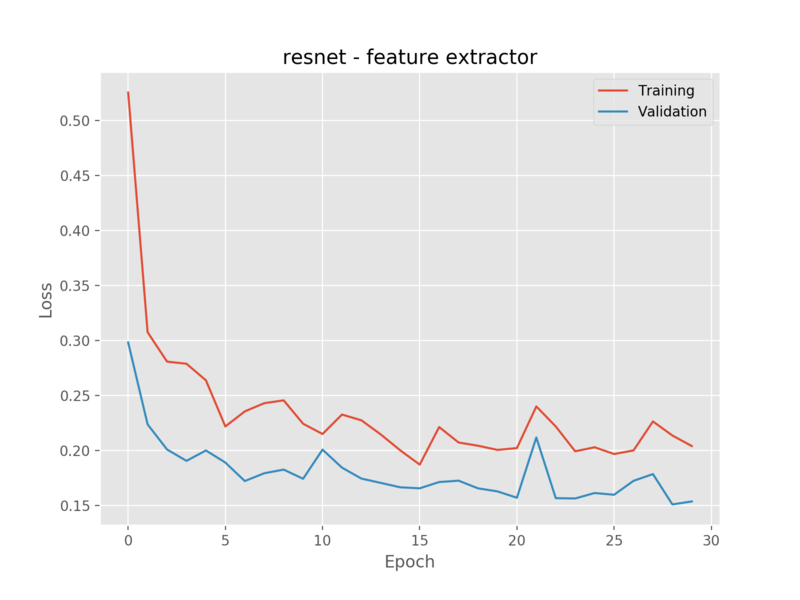
\includegraphics[width=7cm]{b_l_resnet_fe}
    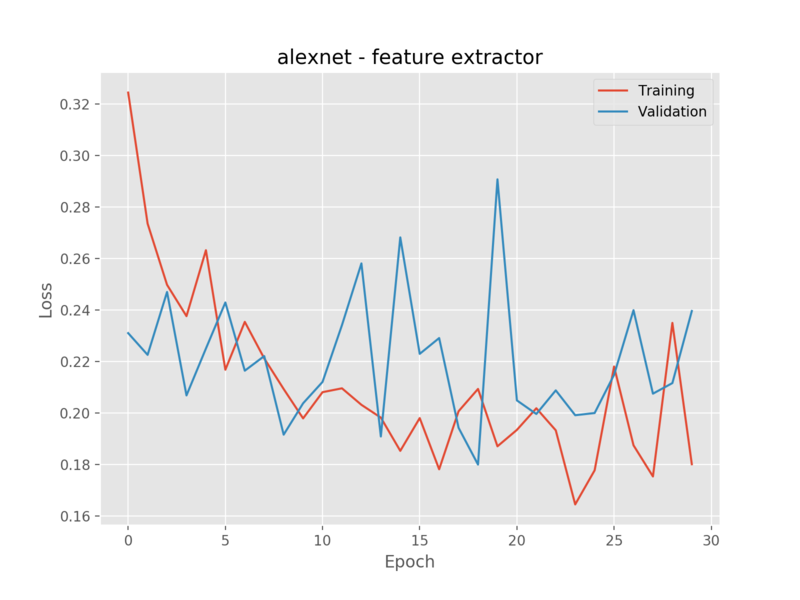
\includegraphics[width=7cm]{b_l_alexnet_fe}
    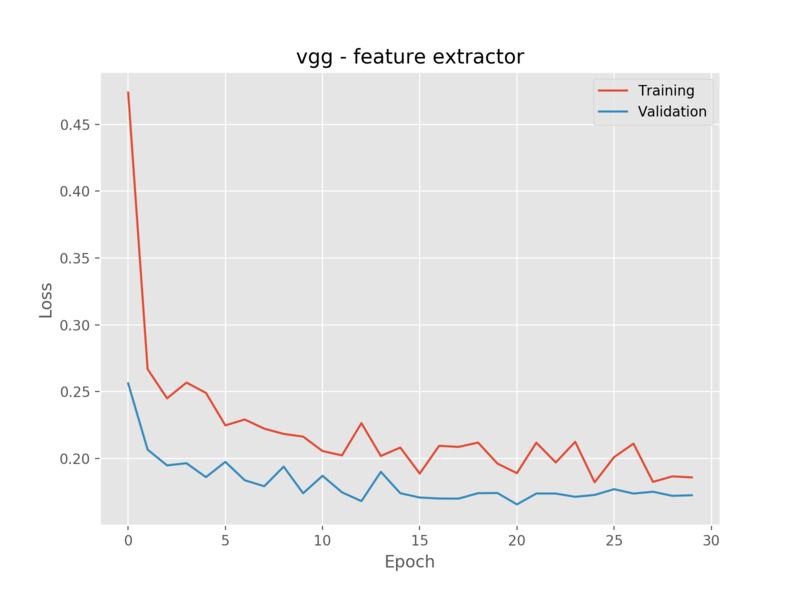
\includegraphics[width=7cm]{b_l_vgg_fe}
    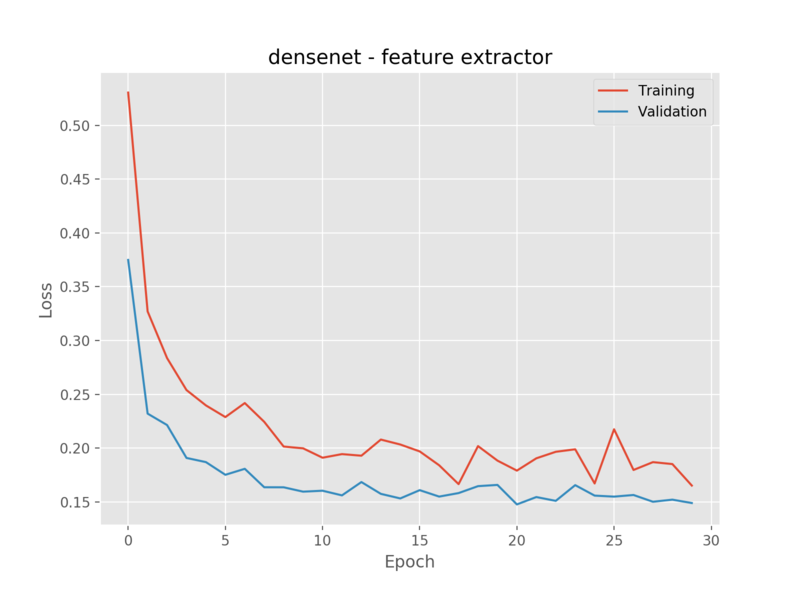
\includegraphics[width=7cm]{b_l_densenet_fe}
    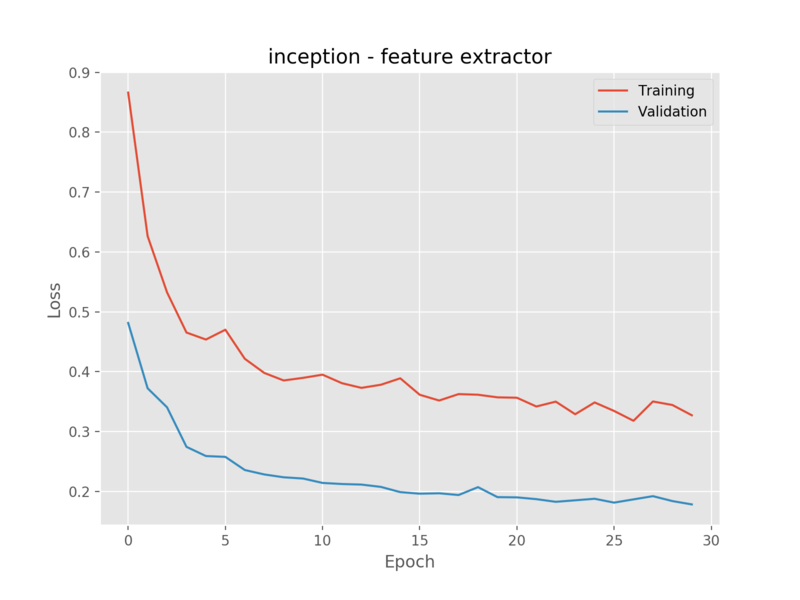
\includegraphics[width=7cm]{b_l_inception_fe}
    \caption{Kostnaden vid varje epoch för balkonger med feature extraction}
    \label{fig:b_l_1}
  \end{figure}
  
  \begin{figure}[h]
    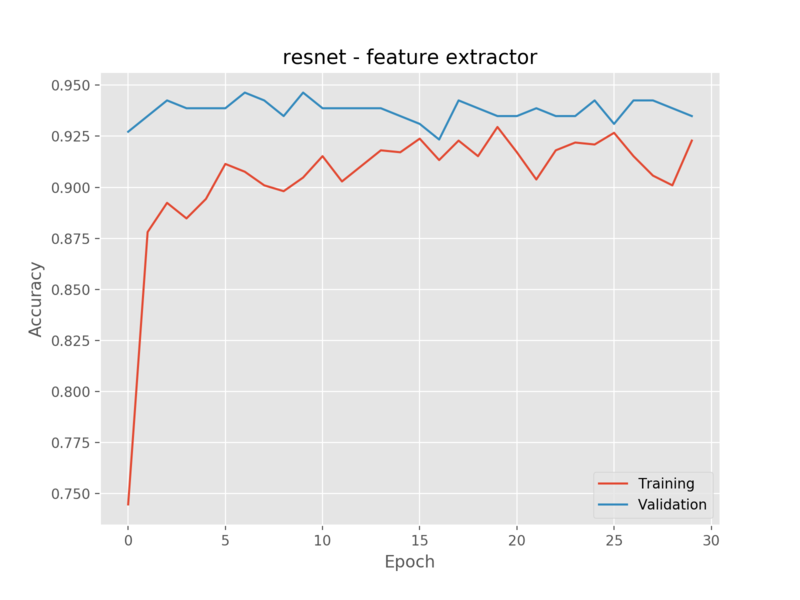
\includegraphics[width=7cm]{b_a_resnet_fe}
    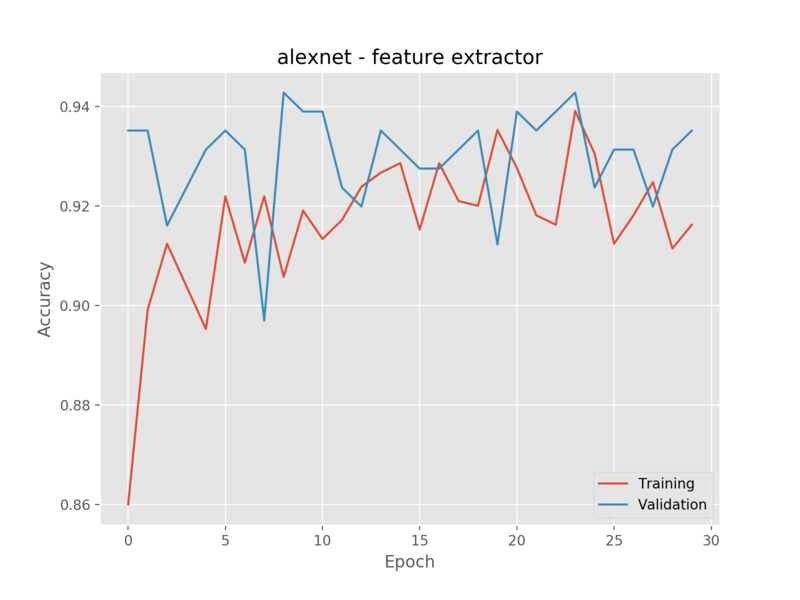
\includegraphics[width=7cm]{b_a_alexnet_fe}
    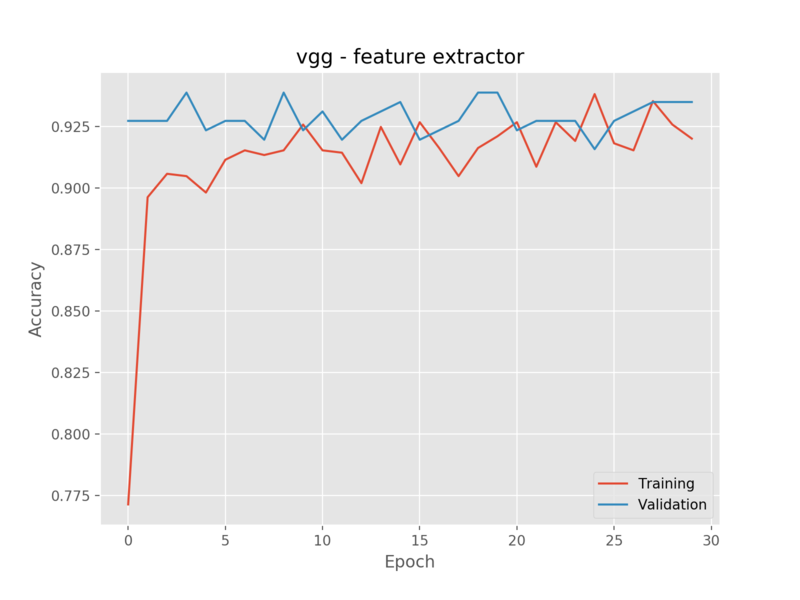
\includegraphics[width=7cm]{b_a_vgg_fe}
    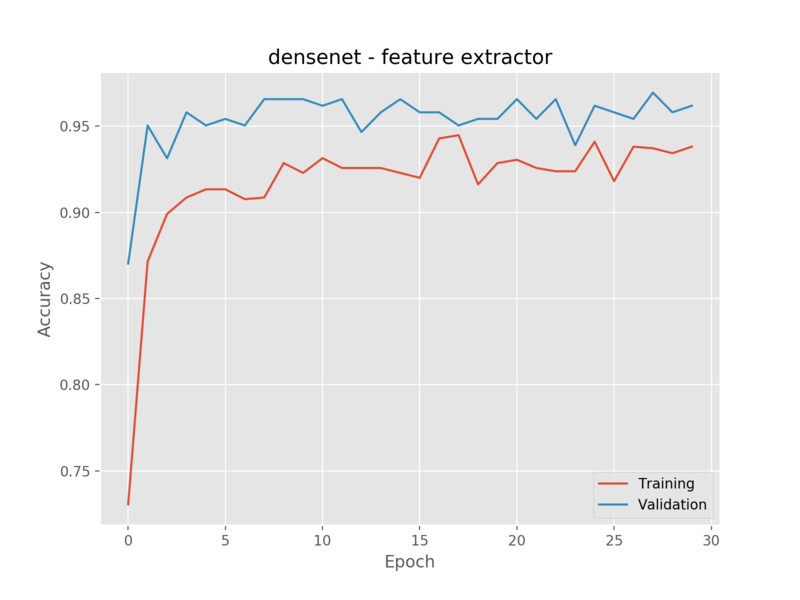
\includegraphics[width=7cm]{b_a_densenet_fe}
    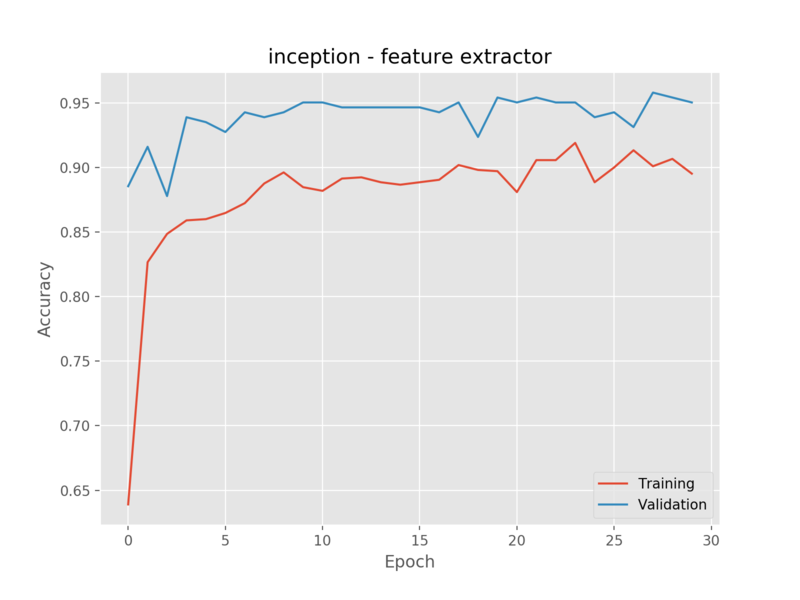
\includegraphics[width=7cm]{b_a_inception_fe}
    \caption{Träffsäkerhet för balkonger med feature extraction}
    \label{fig:b_a_1}
  \end{figure}
  
  \begin{figure}[h]
    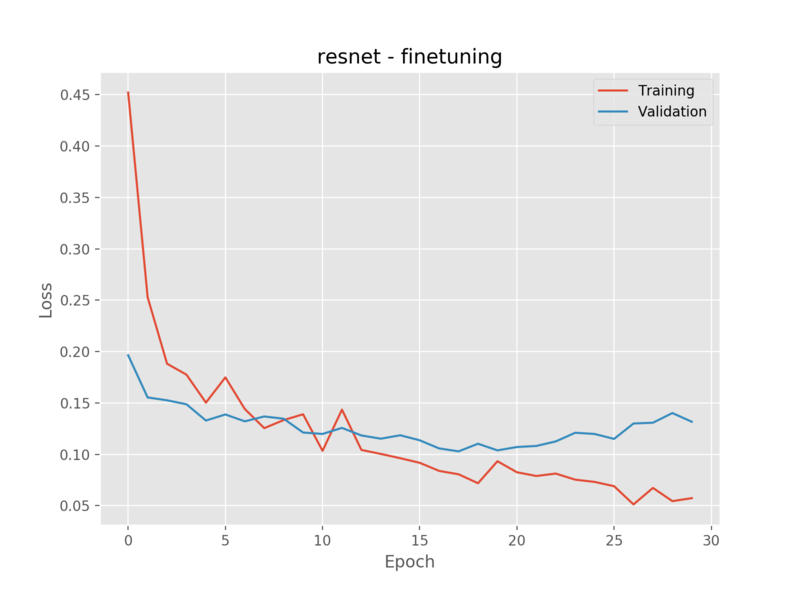
\includegraphics[width=7cm]{b_l_resnet_fine}
    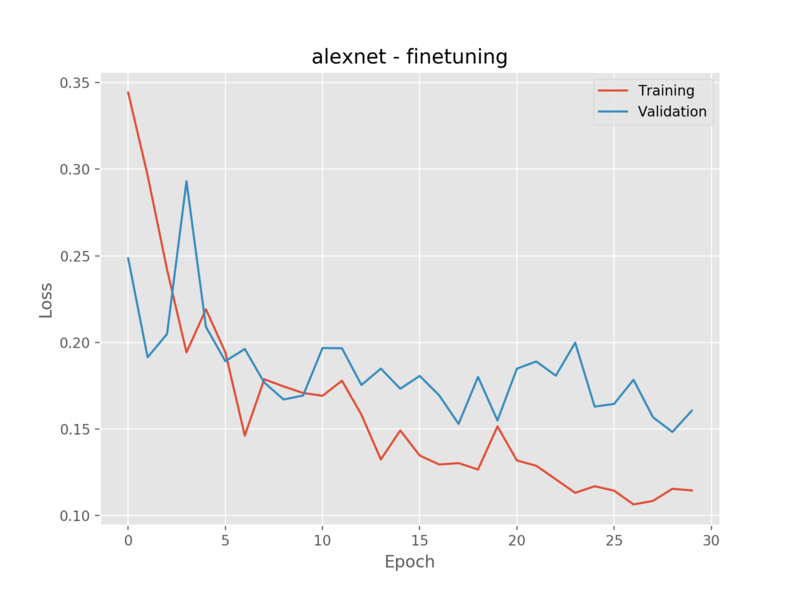
\includegraphics[width=7cm]{b_l_alexnet_fine}
    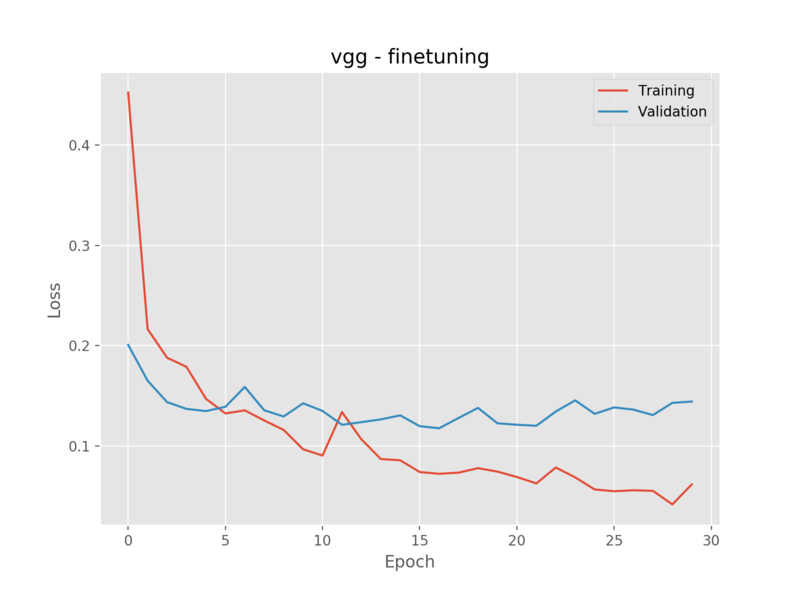
\includegraphics[width=7cm]{b_l_vgg_fine}
    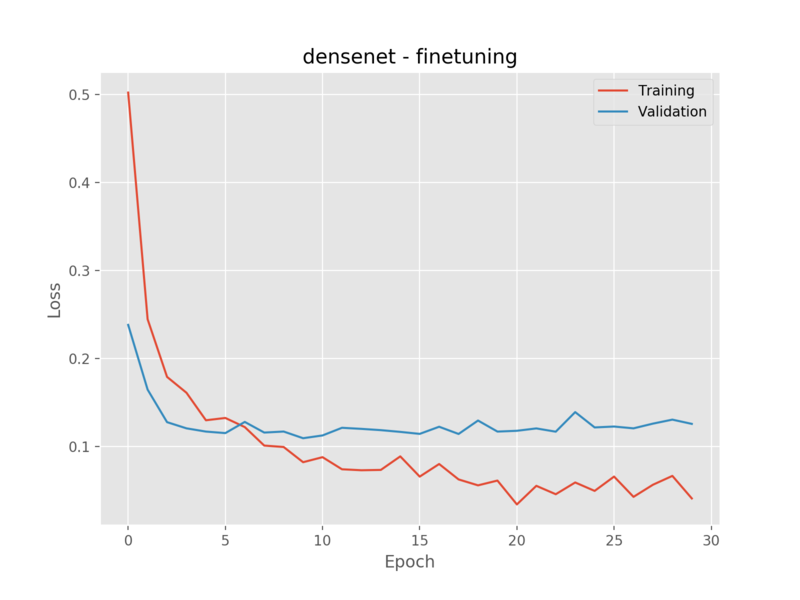
\includegraphics[width=7cm]{b_l_densenet_fine}
    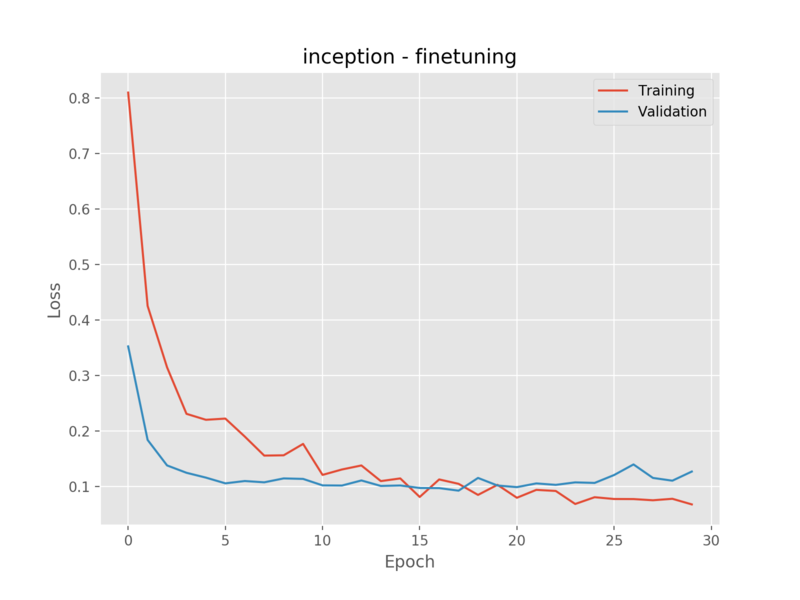
\includegraphics[width=7cm]{b_l_inception_fine}
    \caption{Kostnaden vid varje epoch för balkonger med finetuning}
    \label{fig:b_l_2}
  \end{figure}
  
  \begin{figure}[h]
    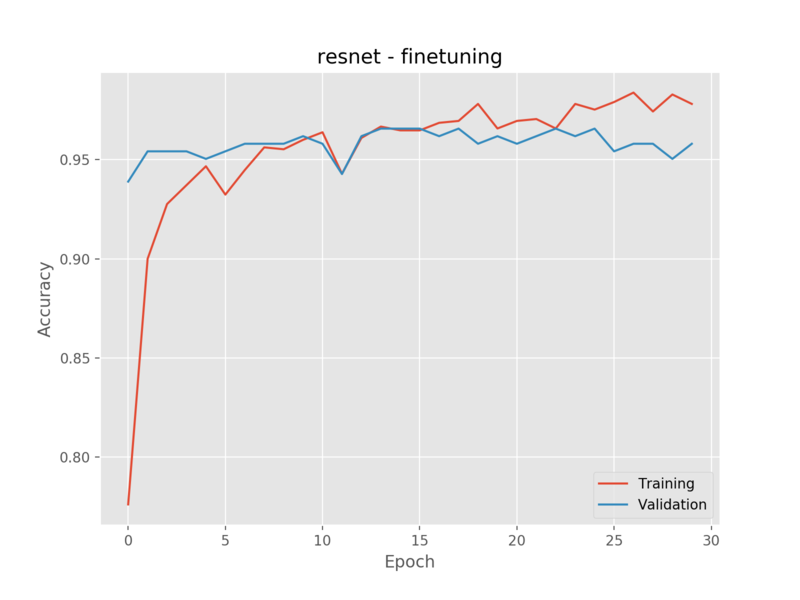
\includegraphics[width=7cm]{b_a_resnet_fine}
    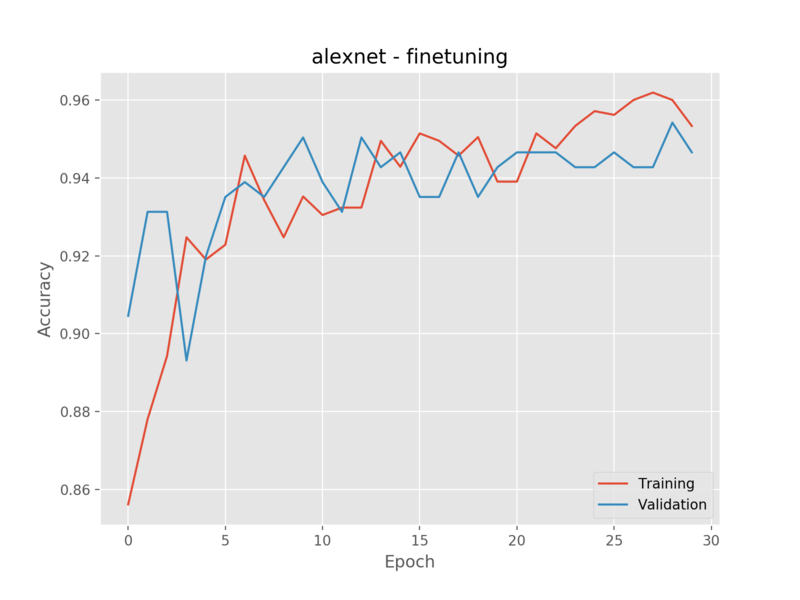
\includegraphics[width=7cm]{b_a_alexnet_fine}
    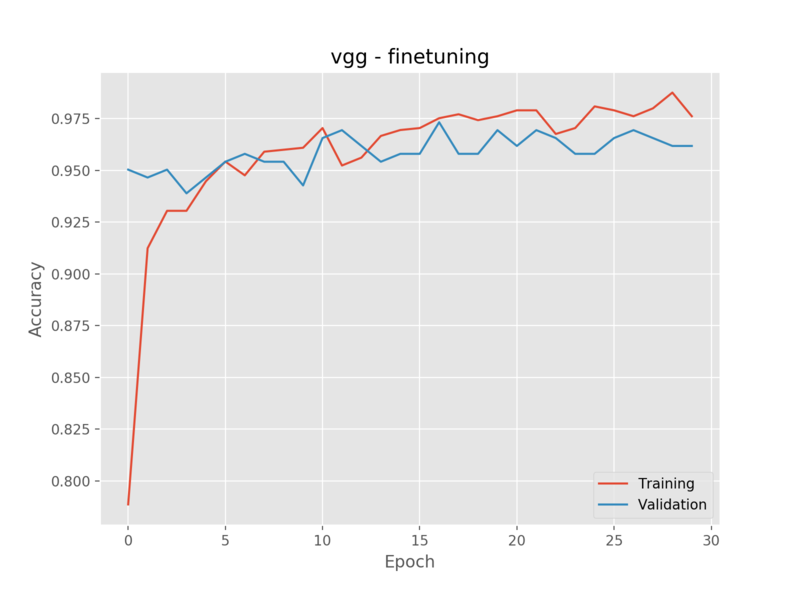
\includegraphics[width=7cm]{b_a_vgg_fine}
    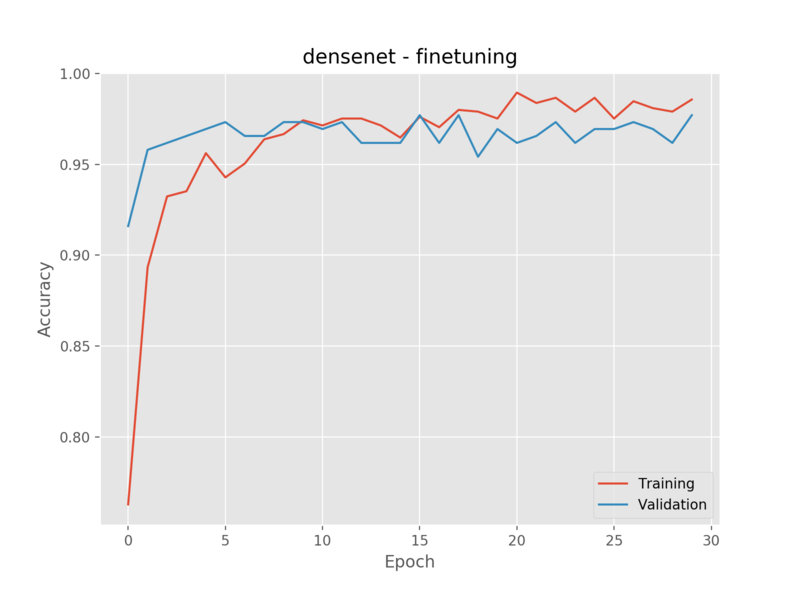
\includegraphics[width=7cm]{b_a_densenet_fine}
    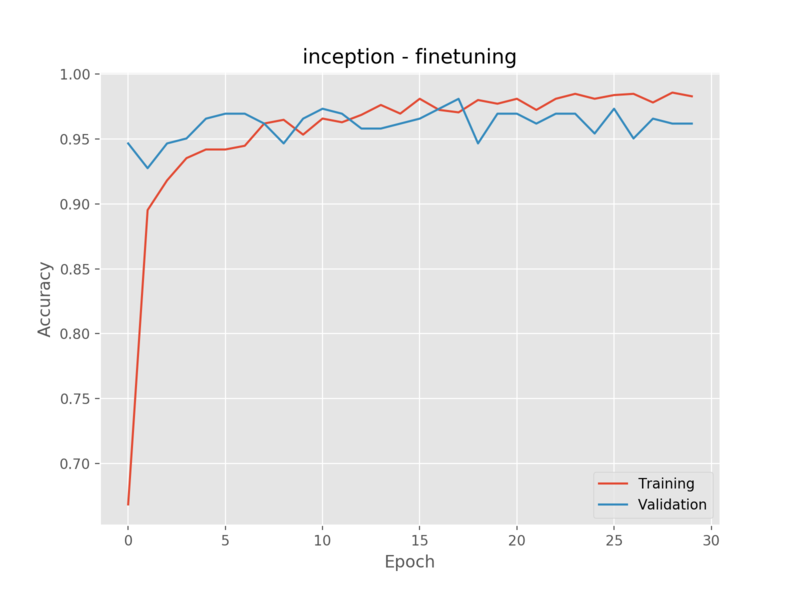
\includegraphics[width=7cm]{b_a_inception_fine}
    \caption{Träffsäkerhet för balkonger med finetuning}
    \label{fig:b_a_2}
  \end{figure}

  \begin{figure}[h]
    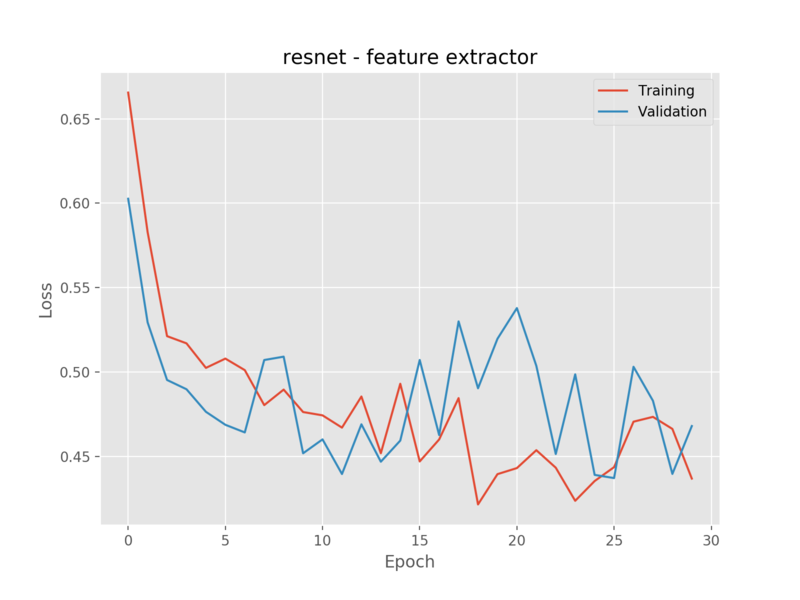
\includegraphics[width=7cm]{f_l_resnet_fe}
    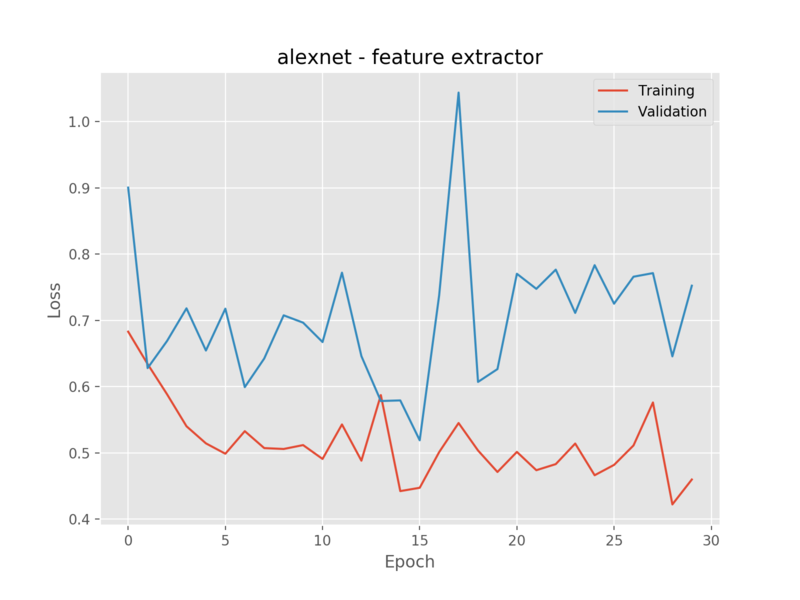
\includegraphics[width=7cm]{f_l_alexnet_fe}
    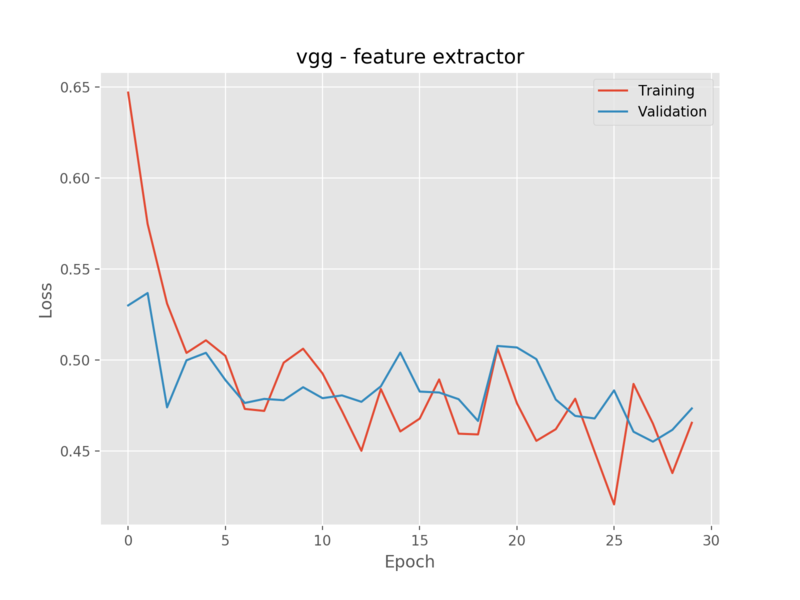
\includegraphics[width=7cm]{f_l_vgg_fe}
    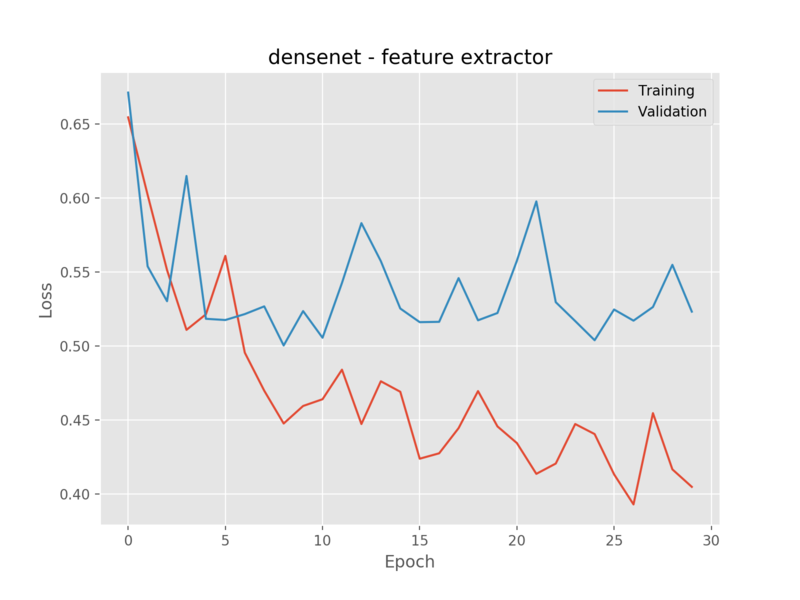
\includegraphics[width=7cm]{f_l_densenet_fe}
    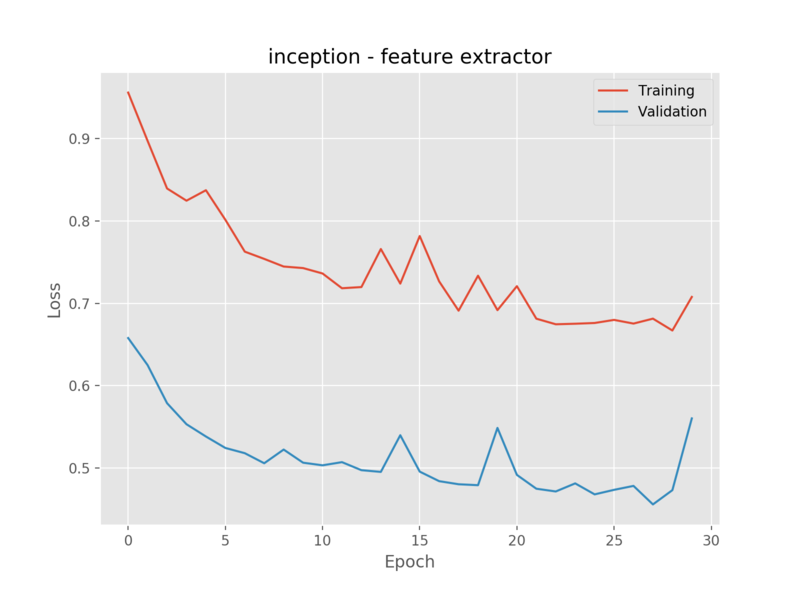
\includegraphics[width=7cm]{f_l_inception_fe}
    \caption{Kostnaden vid varje epoch för eldstäder med feature extraction}
    \label{fig:f_l_1}
  \end{figure}
  
  \begin{figure}[h]
    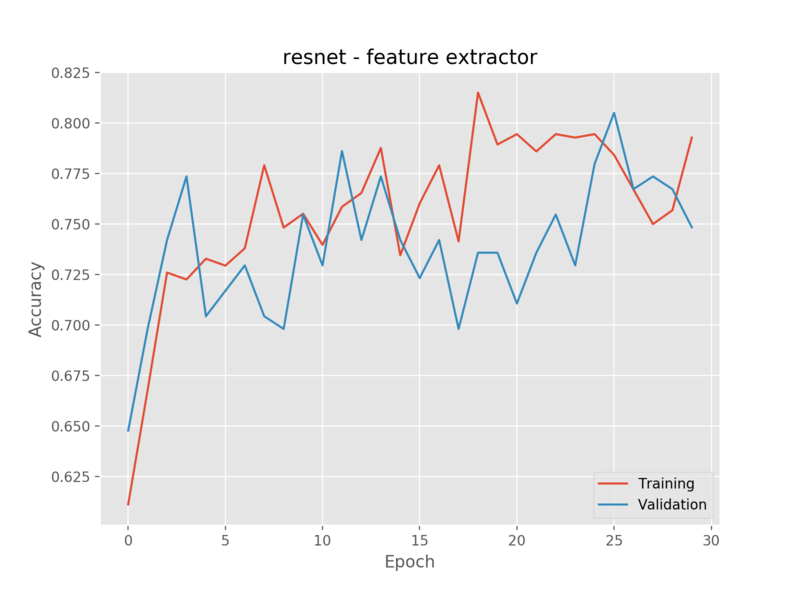
\includegraphics[width=7cm]{f_a_resnet_fe}
    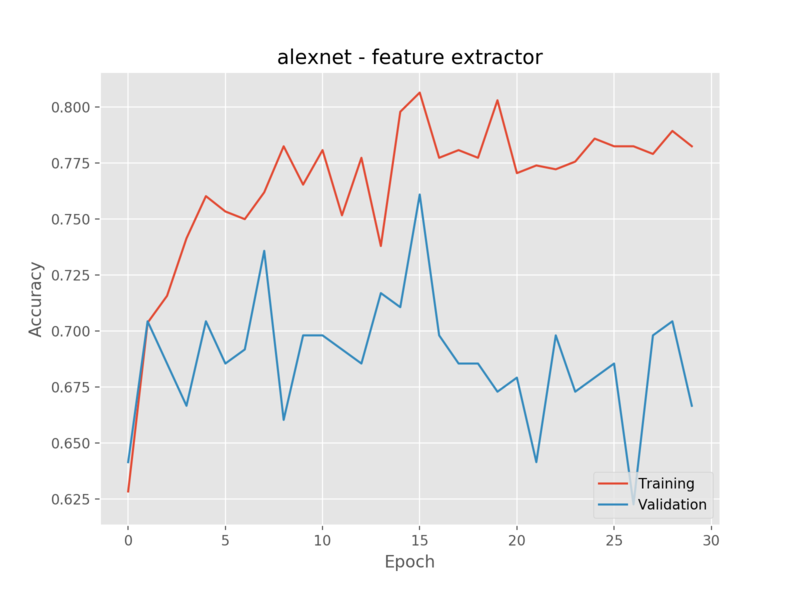
\includegraphics[width=7cm]{f_a_alexnet_fe}
    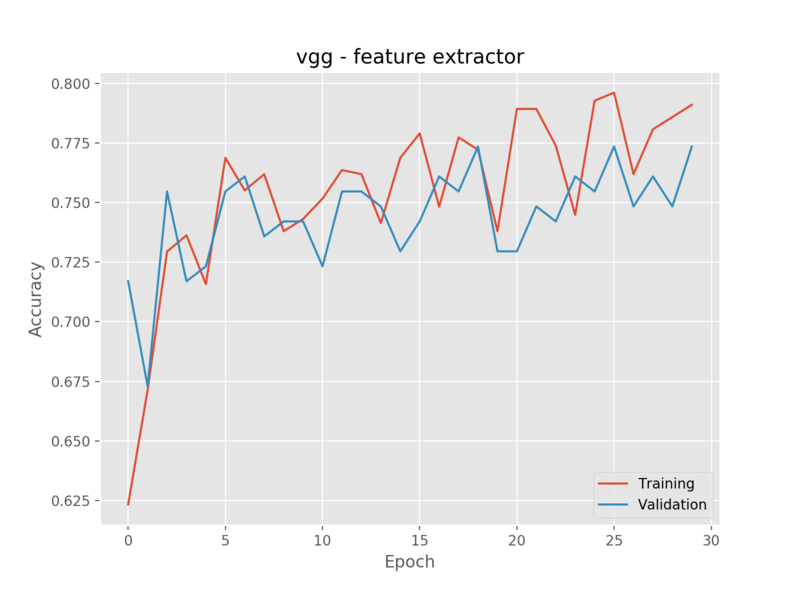
\includegraphics[width=7cm]{f_a_vgg_fe}
    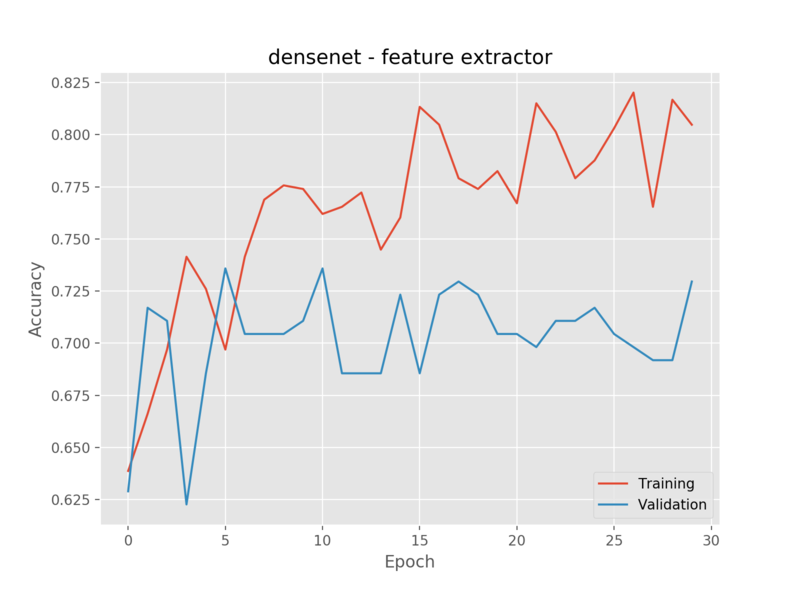
\includegraphics[width=7cm]{f_a_densenet_fe}
    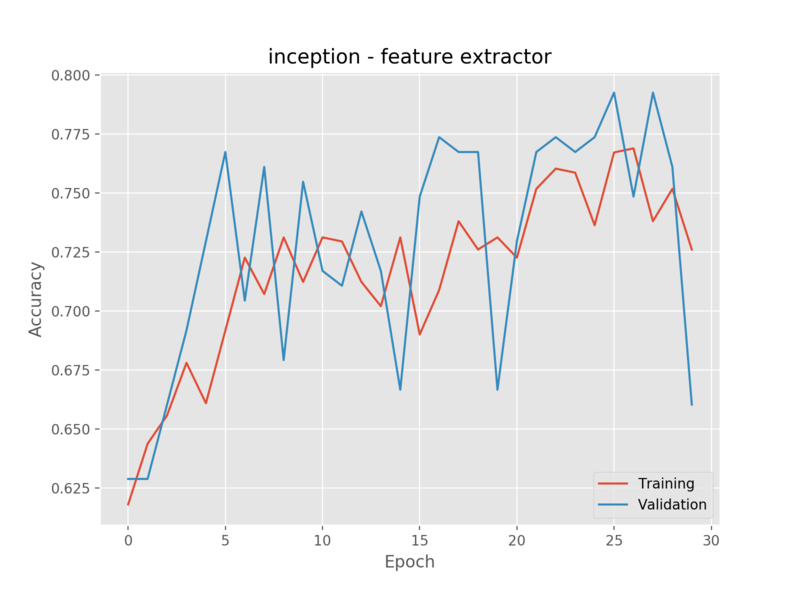
\includegraphics[width=7cm]{f_a_inception_fe}
    \caption{Träffsäkerhet för eldstäder med feature extraction}
    \label{fig:f_a_1}
  \end{figure}

  \begin{figure}[h]
    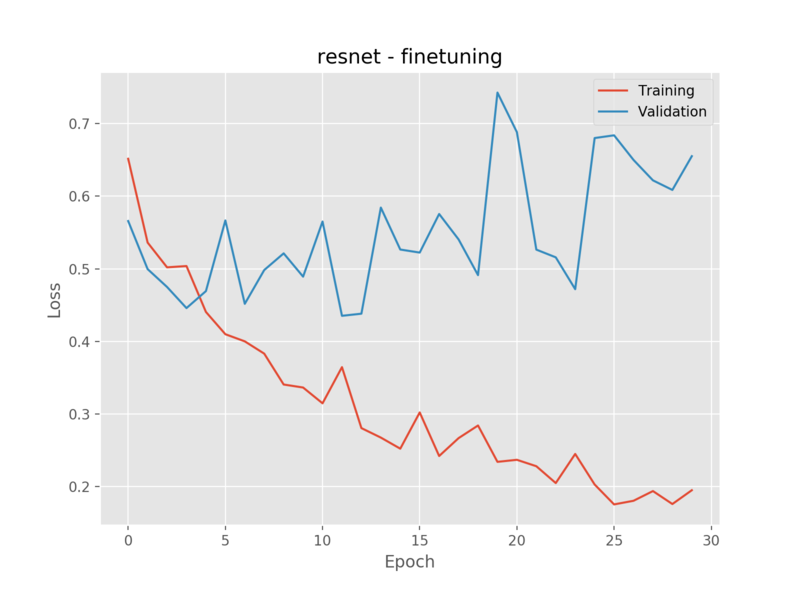
\includegraphics[width=7cm]{f_l_resnet_fine}
    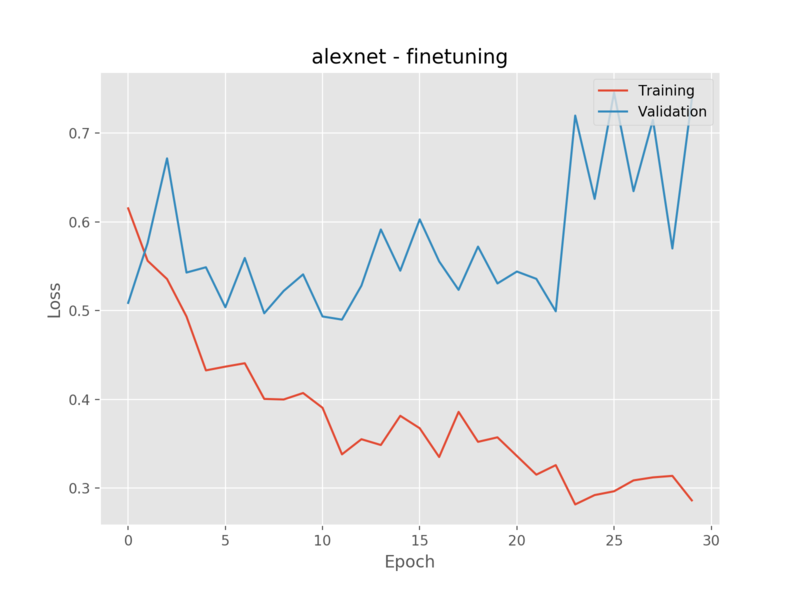
\includegraphics[width=7cm]{f_l_alexnet_fine}
    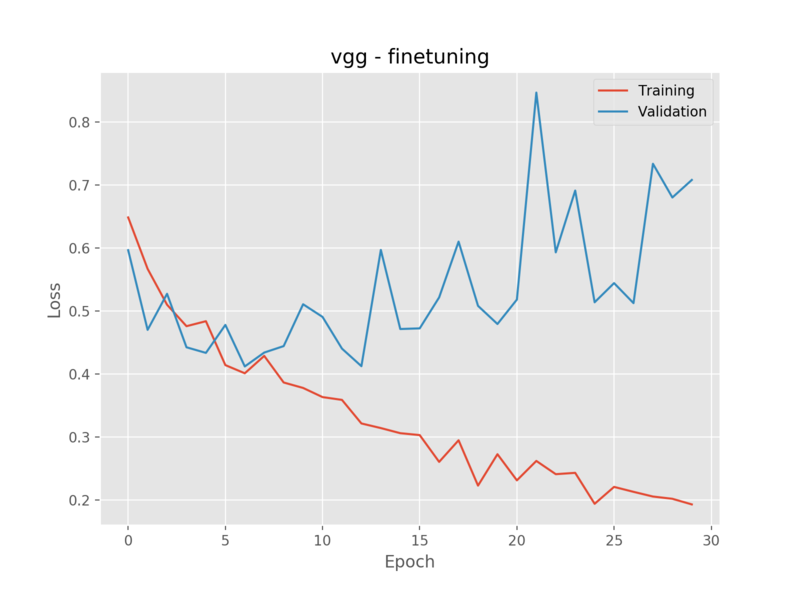
\includegraphics[width=7cm]{f_l_vgg_fine}
    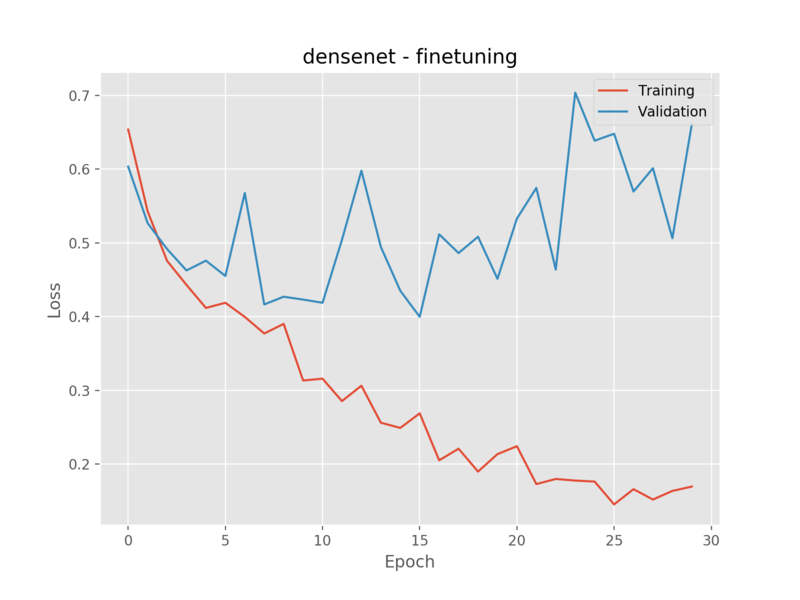
\includegraphics[width=7cm]{f_l_densenet_fine}
    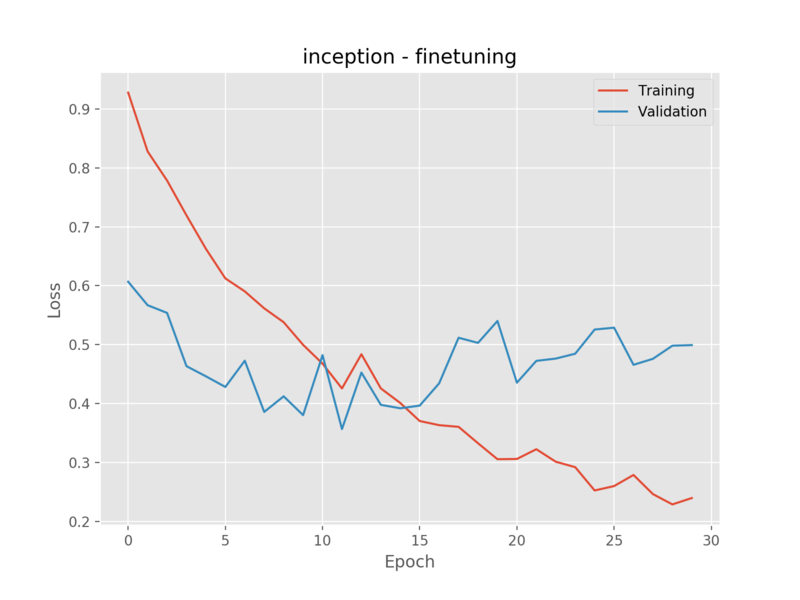
\includegraphics[width=7cm]{f_l_inception_fine}
    \caption{Kostnaden vid varje epoch för eldstäder med finetuning}
    \label{fig:f_l_2}
  \end{figure}

  \begin{figure}[h]
    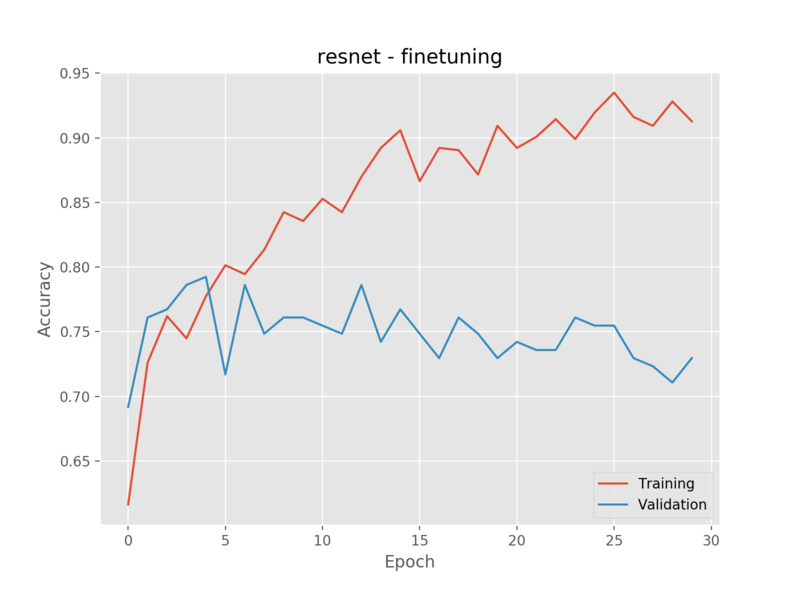
\includegraphics[width=7cm]{f_a_resnet_fine}
    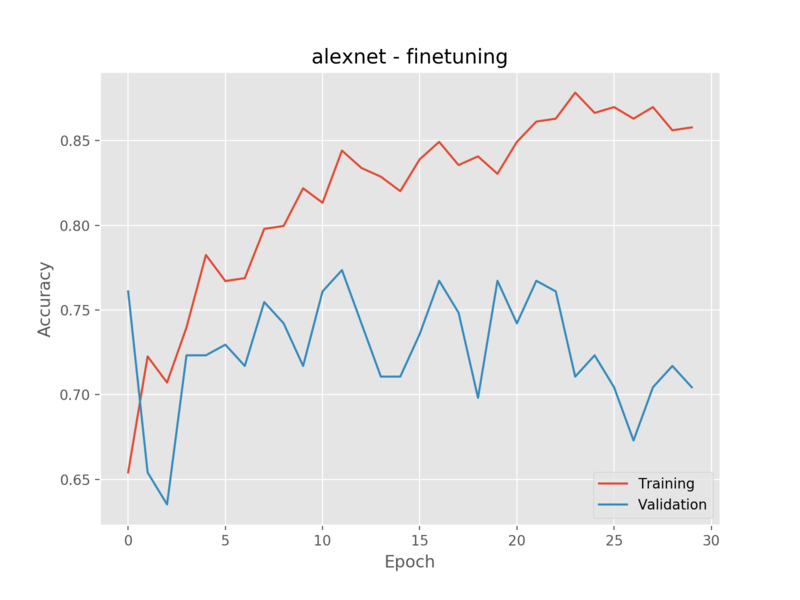
\includegraphics[width=7cm]{f_a_alexnet_fine}
    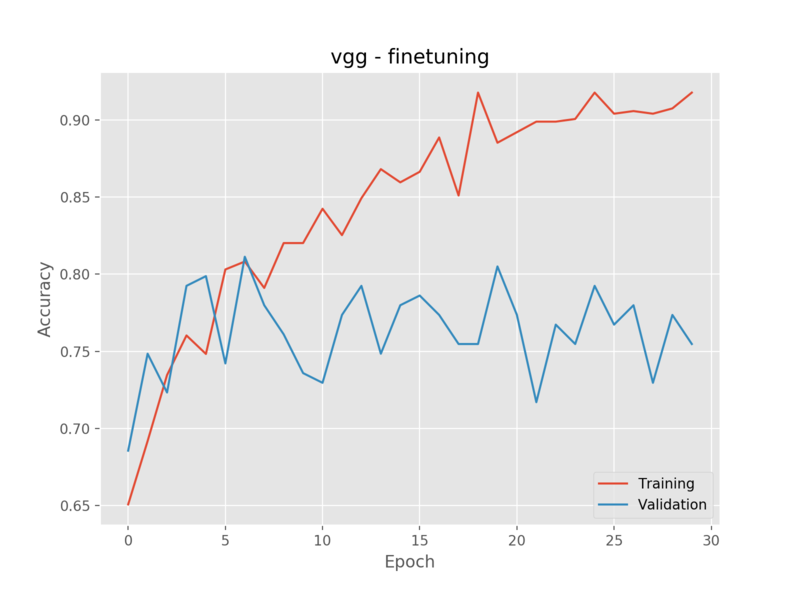
\includegraphics[width=7cm]{f_a_vgg_fine}
    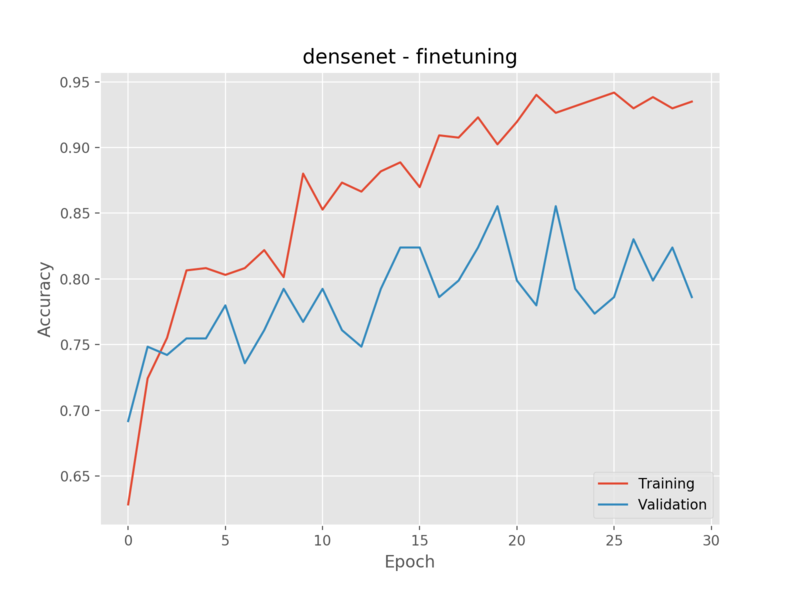
\includegraphics[width=7cm]{f_a_densenet_fine}
    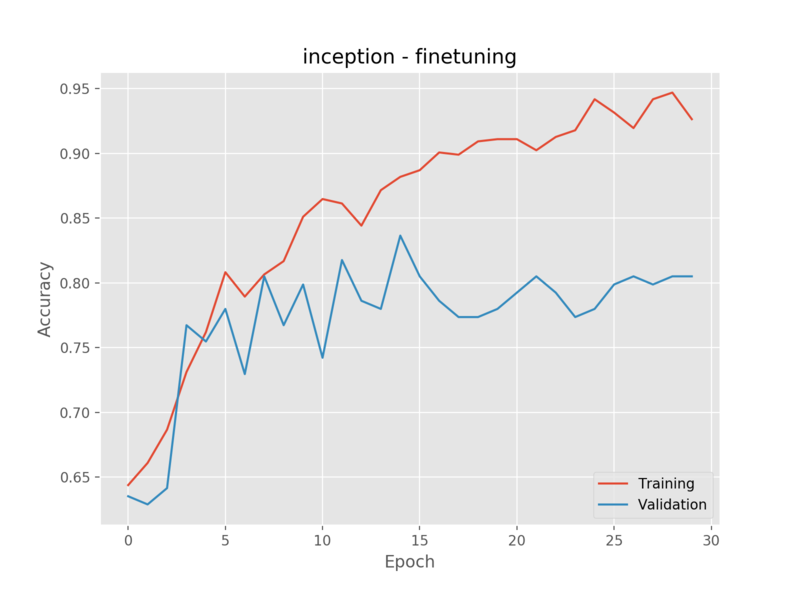
\includegraphics[width=7cm]{f_a_inception_fine}
    \caption{Träffsäkerhet för eldstäder med finetuning}
    \label{fig:f_a_2}
  \end{figure}
  
  \begin{figure}[h]
    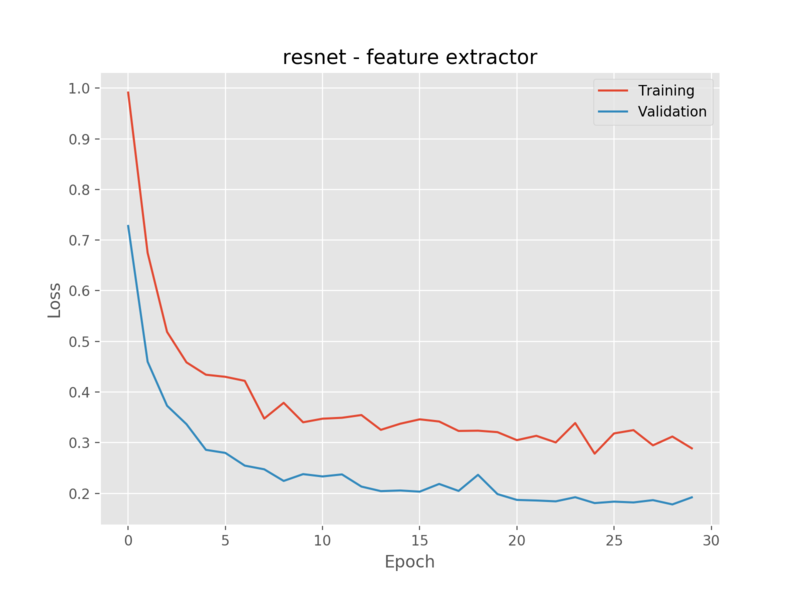
\includegraphics[width=7cm]{r_l_resnet_fe}
    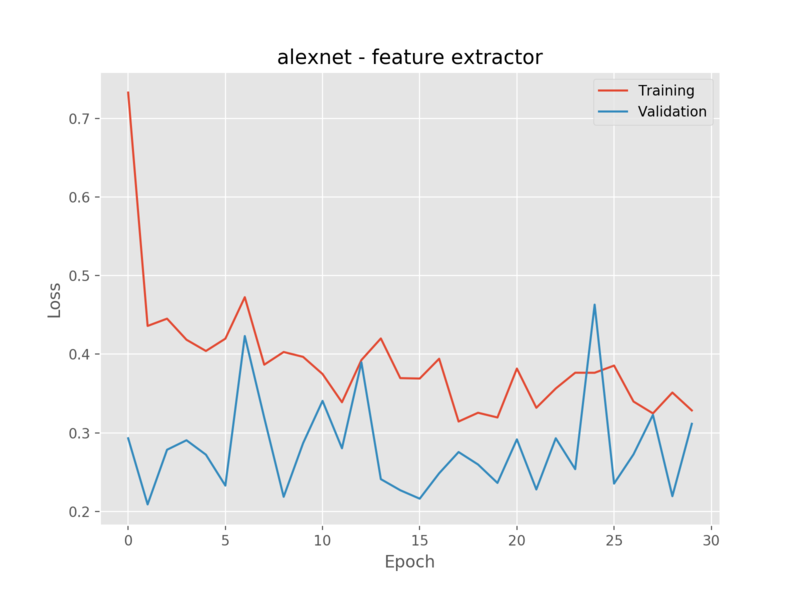
\includegraphics[width=7cm]{r_l_alexnet_fe}
    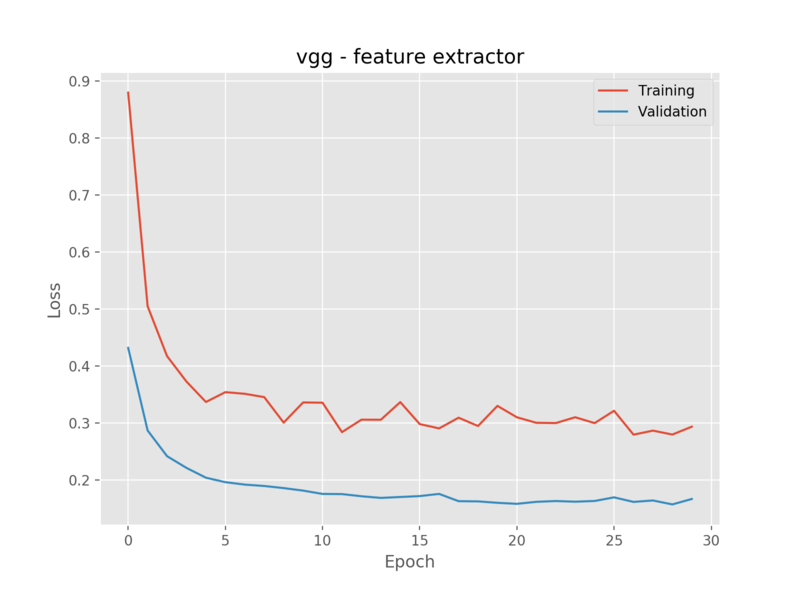
\includegraphics[width=7cm]{r_l_vgg_fe}
    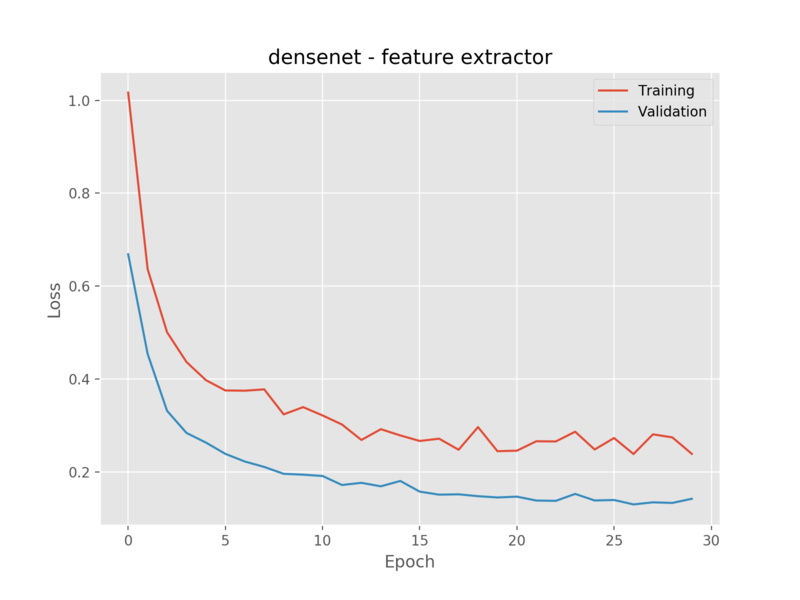
\includegraphics[width=7cm]{r_l_densenet_fe}
    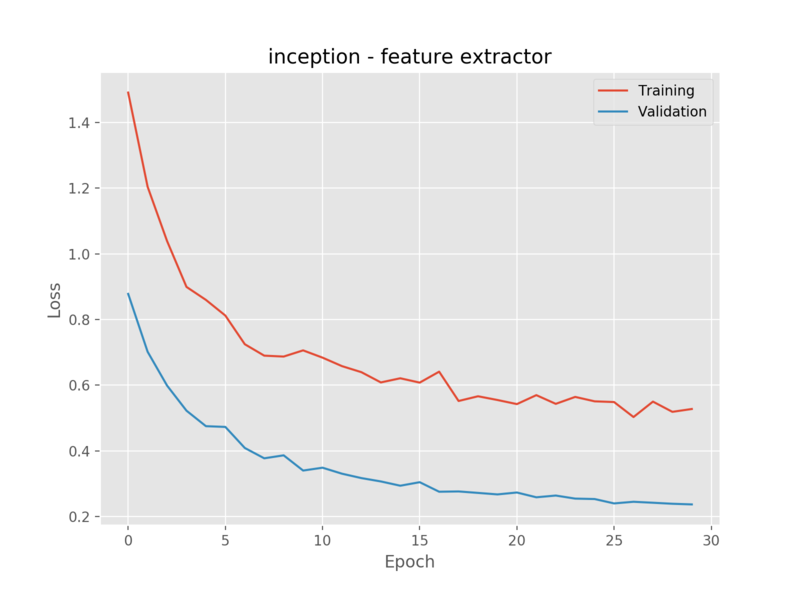
\includegraphics[width=7cm]{r_l_inception_fe}
    \caption{Kostnaden vid varje epoch för rum med feature extraction}
    \label{fig:r_l_1}
  \end{figure}
  
  \begin{figure}[h]
    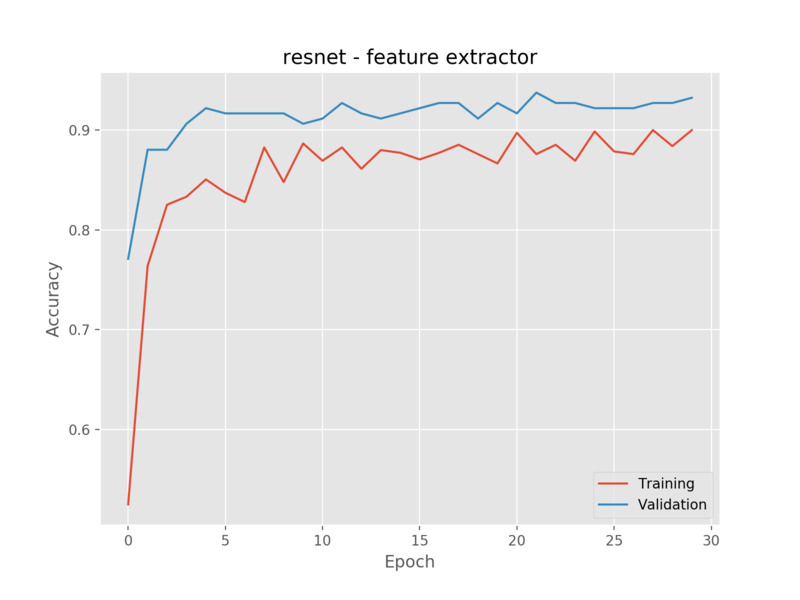
\includegraphics[width=7cm]{r_a_resnet_fe}
    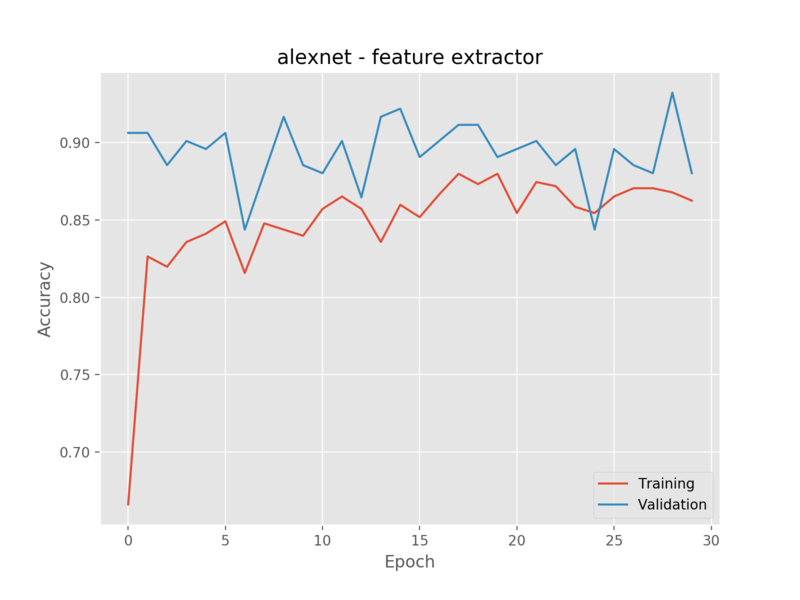
\includegraphics[width=7cm]{r_a_alexnet_fe}
    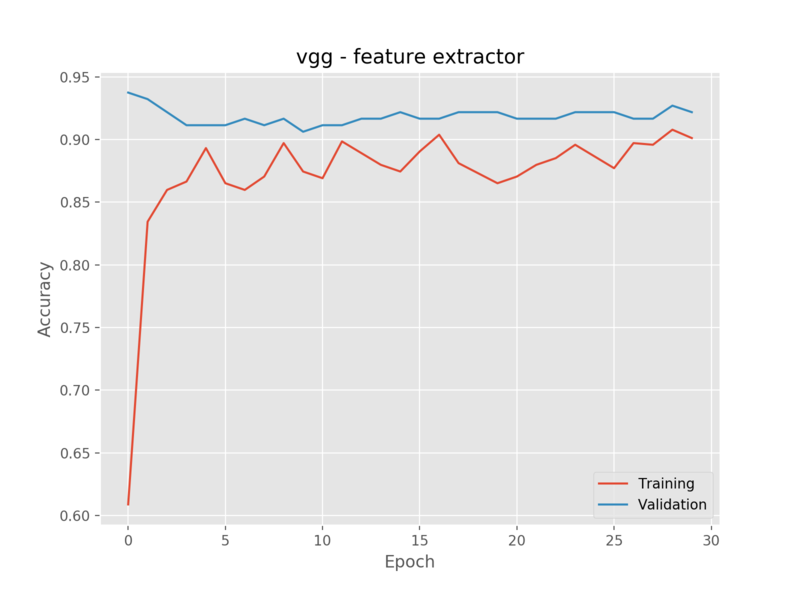
\includegraphics[width=7cm]{r_a_vgg_fe}
    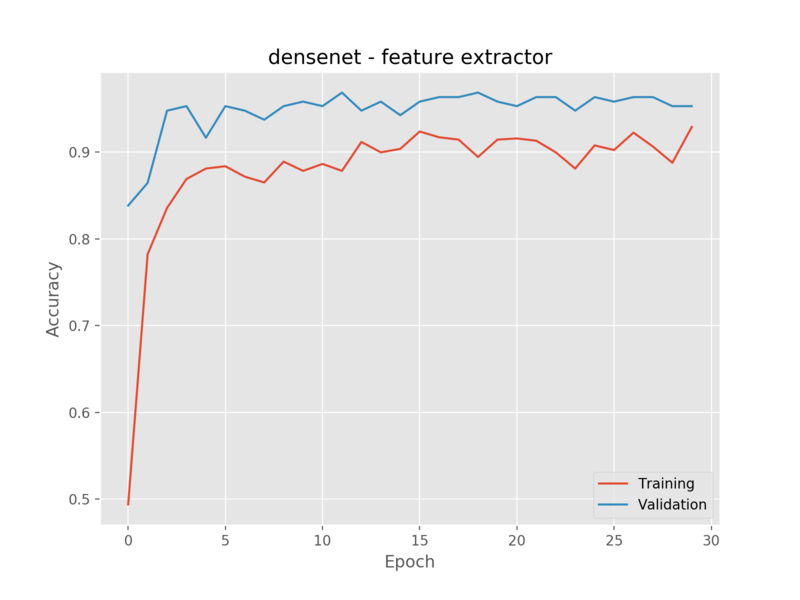
\includegraphics[width=7cm]{r_a_densenet_fe}
    \includegraphics[width=7cm]{r_a_inception_fe}
    \caption{Träffsäkerhet för rum med feature extraction}
    \label{fig:r_a_1}
  \end{figure}
  
  \begin{figure}[h]
    \includegraphics[width=7cm]{r_l_resnet_fine}
    \includegraphics[width=7cm]{r_l_alexnet_fine}
    \includegraphics[width=7cm]{r_l_vgg_fine}
    \includegraphics[width=7cm]{r_l_densenet_fine}
    \includegraphics[width=7cm]{r_l_inception_fine}
    \caption{Kostnaden vid varje epoch för rum med finetuning}
    \label{fig:r_l_2}
  \end{figure}
  
  \begin{figure}[h]
    \includegraphics[width=7cm]{r_a_resnet_fine}
    \includegraphics[width=7cm]{r_a_alexnet_fine}
    \includegraphics[width=7cm]{r_a_vgg_fine}
    \includegraphics[width=7cm]{r_a_densenet_fine}
    \includegraphics[width=7cm]{r_a_inception_fine}
    \caption{Träffsäkerhet för rum med finetuning}
    \label{fig:r_a_2}
  \end{figure}

\tailmatter
\end{document}
